\documentclass[11pt,a4paper]{article}

% ── Packages ─────────────────────────────────────────────────
\usepackage[utf8]{inputenc}
\usepackage[T1]{fontenc}
\usepackage{lmodern}
\usepackage[margin=2.5cm]{geometry}
\usepackage{graphicx}
\usepackage{amsmath,amssymb}
\usepackage{booktabs}
\usepackage{hyperref}
\usepackage{xcolor}
\usepackage{listings}
\usepackage{tikz}
\usetikzlibrary{shapes.geometric, arrows.meta, positioning, calc}
\usepackage{enumitem}
\usepackage{fancyhdr}
\usepackage{titlesec}
\usepackage[labelfont=bf]{caption}
\usepackage{float}
\usepackage{multirow}
\usepackage{subcaption}
\usepackage{makecell}

% ── Colours ──────────────────────────────────────────────────
\definecolor{parnblue}{RGB}{41,98,255}
\definecolor{parngreen}{RGB}{0,150,80}
\definecolor{parngray}{RGB}{100,100,100}
\definecolor{codebg}{RGB}{245,245,248}
\definecolor{codeframe}{RGB}{200,200,210}
\definecolor{stringcolor}{RGB}{163,21,21}
\definecolor{commentcolor}{RGB}{0,128,0}
\definecolor{keywordcolor}{RGB}{0,0,200}

% ── Hyperref ─────────────────────────────────────────────────
\hypersetup{
  colorlinks=true,
  linkcolor=parnblue,
  urlcolor=parnblue,
  citecolor=parnblue,
  pdftitle={Parnassus: Neural Fast Simulation for High Energy Physics},
  pdfauthor={Etienne Dreyer, Eilam Gross, Dmitrii Kobylianskii, Vinicius Mikuni, Benjamin Nachman},
}

% ── Listings ─────────────────────────────────────────────────
\lstset{
  basicstyle=\ttfamily\small,
  backgroundcolor=\color{codebg},
  frame=single,
  rulecolor=\color{codeframe},
  breaklines=true,
  breakatwhitespace=false,
  showstringspaces=false,
  tabsize=2,
  captionpos=b,
  aboveskip=10pt,
  belowskip=10pt,
  xleftmargin=4pt,
  xrightmargin=4pt,
  framexleftmargin=4pt,
  framexrightmargin=4pt,
}

\lstdefinestyle{bash}{
  language=bash,
  morekeywords={parnassus,pip,git,cd},
  keywordstyle=\color{keywordcolor}\bfseries,
  commentstyle=\color{commentcolor}\itshape,
  stringstyle=\color{stringcolor},
}

\lstdefinestyle{python}{
  language=Python,
  keywordstyle=\color{keywordcolor}\bfseries,
  commentstyle=\color{commentcolor}\itshape,
  stringstyle=\color{stringcolor},
  morekeywords={Path,Config,GenerationPipeline,JetClusteringPipeline,
    IsolationPipeline,JetClusteringConfig,IsolationConfig,
    RootWriter,HepMC3Generator,self},
}

\lstdefinestyle{yaml}{
  basicstyle=\ttfamily\small,
  backgroundcolor=\color{codebg},
  frame=single,
  rulecolor=\color{codeframe},
  breaklines=true,
  showstringspaces=false,
  commentstyle=\color{commentcolor}\itshape,
  morecomment=[l]{\#},
}

\lstdefinestyle{cmnd}{
  basicstyle=\ttfamily\small,
  backgroundcolor=\color{codebg},
  frame=single,
  rulecolor=\color{codeframe},
  breaklines=true,
  showstringspaces=false,
  commentstyle=\color{commentcolor}\itshape,
  morecomment=[l]{!},
}

% ── Headers ──────────────────────────────────────────────────
\pagestyle{fancy}
\fancyhf{}
\fancyhead[L]{\small\textsc{Parnassus} v0.1.0}
\fancyhead[R]{\small Product Reference Document}
\fancyfoot[C]{\thepage}
\renewcommand{\headrulewidth}{0.4pt}

% ── Title formatting ────────────────────────────────────────
\titleformat{\section}{\Large\bfseries\color{parnblue}}{\thesection}{1em}{}
\titleformat{\subsection}{\large\bfseries\color{parnblue!80!black}}{\thesubsection}{1em}{}
\titleformat{\subsubsection}{\normalsize\bfseries}{\thesubsubsection}{1em}{}

% ══════════════════════════════════════════════════════════════
\begin{document}

% ── Title page ───────────────────────────────────────────────
\begin{titlepage}
\centering
\vspace*{3cm}
{\Huge\bfseries\color{parnblue} Parnassus\par}
\vspace{0.5cm}
{\LARGE Neural Fast Simulation for\\High Energy Physics\par}
\vspace{2cm}
{\Large Product Reference Document\par}
\vspace{0.5cm}
{\large Version 0.1.0\par}
\vspace{2cm}
{\large
  Etienne Dreyer$^{1}$,\quad
  Eilam Gross$^{1}$,\quad
  Dmitrii Kobylianskii$^{1}$,\quad
  Vinicius Mikuni$^{2}$,\quad
  Benjamin Nachman$^{2}$\par}
\vspace{0.5cm}
{\small
  $^{1}$Weizmann Institute of Science, Rehovot, Israel\\[4pt]
  $^{2}$Lawrence Berkeley National Laboratory, Berkeley, CA, USA\par}
\vspace{3cm}
{\large\today\par}
\vfill
{\small Licensed under the MIT License}
\end{titlepage}

% ── Table of Contents ────────────────────────────────────────
\tableofcontents
\newpage

% ══════════════════════════════════════════════════════════════
\section{Introduction}
\label{sec:introduction}

Parnassus is a Python framework for fast detector simulation in High Energy Physics (HEP).
It replaces the computationally expensive full \textsc{Geant4} simulation chain with neural
network-based generative models that learn the mapping from truth-level (generator-level)
particles to detector-level particle-flow (pflow) objects. The framework is
\textbf{process-agnostic}: the same pre-trained models can be applied to arbitrary physics
processes by simply providing different input truth events.

\subsection{Design Goals}

\begin{description}[style=nextline,leftmargin=2.5cm]
  \item[\textbf{Speed}] Orders of magnitude faster than full simulation by replacing the
    detector response with neural diffusion models.
  \item[\textbf{Fidelity}] Trained on real CMS 2011 data to reproduce realistic
    detector-level distributions including particle kinematics, vertex positions,
    impact parameters, and particle identification.
  \item[\textbf{Flexibility}] Accept truth-level input from any source --- \textsc{Pythia8}
    on-the-fly generation, HepMC files from external generators (\textsc{MadGraph},
    \textsc{Sherpa}, \textsc{Herwig}, \textsc{Powheg}), or custom formats.
  \item[\textbf{Completeness}] Full post-processing pipeline including jet clustering
    (\textsc{FastJet}) and lepton isolation, with output to ROOT format.
\end{description}

\subsection{What Parnassus Produces}

Given a set of truth-level particles for each event, Parnassus generates the quantities
listed in Table~\ref{tab:outputs}.

\begin{table}[H]
\centering
\caption{Output quantities produced by Parnassus for each event.}
\label{tab:outputs}
\begin{tabular}{@{}ll@{}}
\toprule
\textbf{Output} & \textbf{Description} \\
\midrule
Particle-flow particles & Full kinematics ($p_\mathrm{T}$, $\eta$, $\phi$), vertex
  ($v_x$, $v_y$, $v_z$), class, PDG\,ID \\
Impact parameters & $d_0$, $z_0$ and their errors for charged particles \\
Jets & Clustered with configurable algorithms (anti-$k_t$, gen-$k_t$);
  substructure ($D_2$, $C_2$) \\
Lepton isolation & Isolation scores and $p_\mathrm{T}$ sums in configurable
  $\Delta R$ cones \\
Event-level quantities & $H_\mathrm{T}$, $\vec{E}_\mathrm{T}^\mathrm{miss}$
  components, particle multiplicity \\
\bottomrule
\end{tabular}
\end{table}

% ══════════════════════════════════════════════════════════════
\section{Architecture Overview}
\label{sec:architecture}

Parnassus uses a three-stage neural generation pipeline followed by physics-based
post-processing. The architecture is illustrated in Figure~\ref{fig:architecture}.

\begin{figure}[H]
\centering
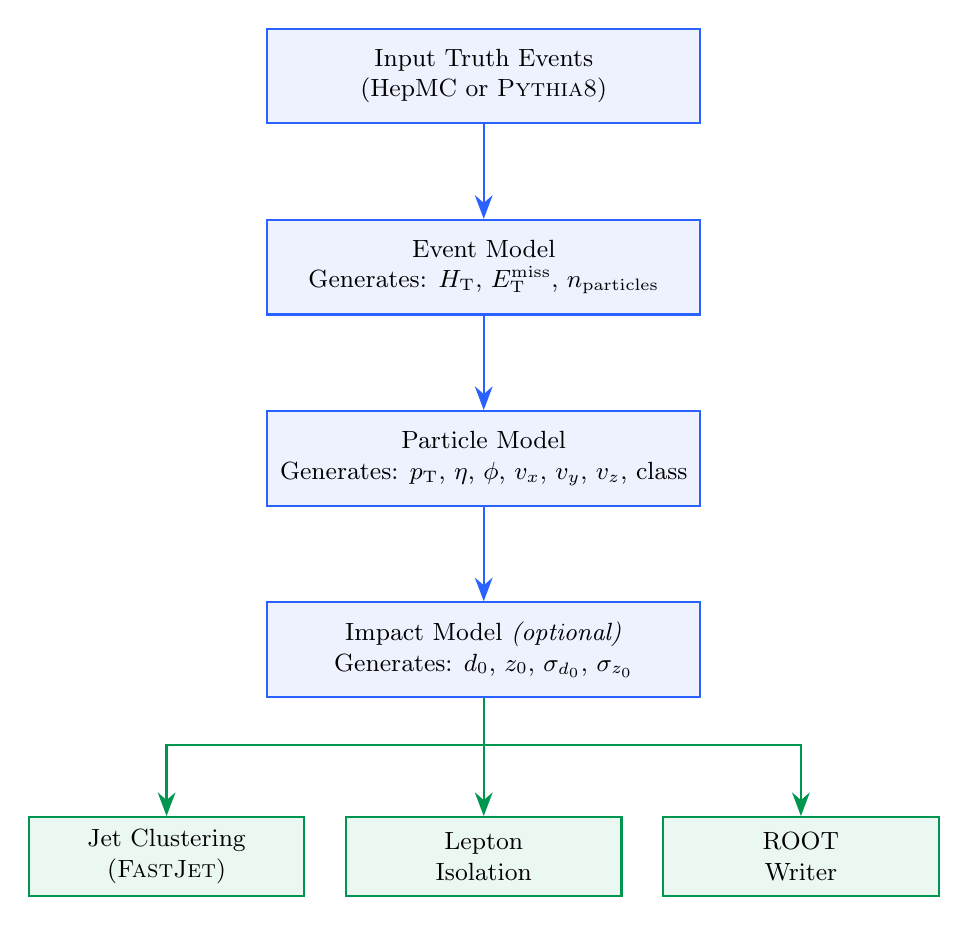
\begin{tikzpicture}[
  node distance=1.2cm,
  box/.style={rectangle, draw=parnblue, fill=parnblue!8, thick,
    minimum width=5.5cm, minimum height=1.2cm, align=center,
    font=\small},
  postbox/.style={rectangle, draw=parngreen, fill=parngreen!8, thick,
    minimum width=3.5cm, minimum height=1.0cm, align=center,
    font=\small},
  arr/.style={-{Stealth[length=3mm]}, thick, parnblue},
  arrg/.style={-{Stealth[length=3mm]}, thick, parngreen},
]
  % Main pipeline
  \node[box] (input) {Input Truth Events\\(HepMC or \textsc{Pythia8})};
  \node[box, below=of input] (event) {Event Model\\
    Generates: $H_\mathrm{T}$, $E_\mathrm{T}^\mathrm{miss}$, $n_\mathrm{particles}$};
  \node[box, below=of event] (particle) {Particle Model\\
    Generates: $p_\mathrm{T}$, $\eta$, $\phi$, $v_x$, $v_y$, $v_z$, class};
  \node[box, below=of particle] (impact) {Impact Model \emph{(optional)}\\
    Generates: $d_0$, $z_0$, $\sigma_{d_0}$, $\sigma_{z_0}$};

  % Arrows
  \draw[arr] (input) -- (event);
  \draw[arr] (event) -- (particle);
  \draw[arr] (particle) -- (impact);

  % Post-processing
  \node[postbox, below left=1.5cm and -0.5cm of impact] (jets) {Jet Clustering\\(\textsc{FastJet})};
  \node[postbox, below=1.5cm of impact] (iso) {Lepton\\Isolation};
  \node[postbox, below right=1.5cm and -0.5cm of impact] (root) {ROOT\\Writer};

  \draw[arrg] (impact.south) -- ++(0,-0.6) -| (jets.north);
  \draw[arrg] (impact.south) -- (iso.north);
  \draw[arrg] (impact.south) -- ++(0,-0.6) -| (root.north);
\end{tikzpicture}
\caption{Parnassus generation pipeline. Three neural diffusion models (blue) produce
  detector-level quantities from truth-level input. Physics-based post-processing
  stages (green) compute derived quantities and write the final output.}
\label{fig:architecture}
\end{figure}

All three neural models are \textbf{diffusion models} sampled via Euler integration.
Each model is conditioned on truth-level particle information, making the generation
process inherently dependent on the input physics process without being tied to any
specific one.

\subsection{Neural Model Details}

Table~\ref{tab:models} summarises the three neural models and their input/output
specifications.

\begin{table}[H]
\centering
\caption{Neural model specifications for the CMS\,2011\,Flow\,v1 generator.}
\label{tab:models}
\begin{tabular}{@{}llll@{}}
\toprule
\textbf{Model} & \textbf{Input Context} & \textbf{Output Variables} & \textbf{Sampler} \\
\midrule
Event & \makecell[l]{Truth particle kinematics\\
  ($p_\mathrm{T}^\mathrm{rel}$, $\eta$, $\phi$, $v_x$, $v_y$, $v_z$, class),\\
  global sums ($H_\mathrm{T}$, MET, $n_\mathrm{truth}$)}
  & \makecell[l]{pflow $H_\mathrm{T}$,\\$\mathrm{MET}_x$, $\mathrm{MET}_y$,\\$n_\mathrm{pflow}$}
  & Euler, 50 steps \\
\addlinespace
Particle & Same + event model outputs
  & \makecell[l]{pflow $p_\mathrm{T}^\mathrm{rel}$, $\eta$, $\phi$,\\$v_x$, $v_y$, $v_z$, class}
  & \makecell[l]{Euler (reverse\\time), 50 steps} \\
\addlinespace
Impact & Same + event model outputs
  & $d_0$, $z_0$, $\sigma_{d_0}$, $\sigma_{z_0}$
  & Euler, 50 steps \\
\bottomrule
\end{tabular}
\end{table}

The number of diffusion steps is configurable at runtime via the \texttt{-{}-num\_steps}
(\texttt{-n}) flag, allowing users to trade generation speed for quality.

% ══════════════════════════════════════════════════════════════
\section{Code Structure}
\label{sec:code-structure}

The source tree is organised into clearly separated modules. The complete layout is shown
below:

\begin{lstlisting}[style=bash,caption={Source tree layout.},label=lst:tree]
src/parnassus/
|-- main.py                    # CLI entry point (init, run)
|-- configs/
|   |-- config.py              # Top-level Config dataclass
|   |-- data.py                # DatasetConfig
|   |-- writer.py              # WriterConfig
|   |-- pipeline.py            # JetClusteringConfig, IsolationConfig
|   |-- scheme.py              # GenEvent, GenParticleCollection, ...
|   |-- accessors.py           # Accessor system for ROOT output
|   |-- variables.py           # VariableRequirements
|   |-- default_config.yaml    # Default configuration template
|   +-- generators/
|       |-- base.py            # GeneratorConfig (ABC)
|       |-- neural.py          # NeuralGeneratorConfig + registry
|       |-- parametric.py      # ParametricGeneratorConfig
|       +-- model.py           # ModelConfig, SamplerConfig
|-- data/
|   |-- base.py                # BaseDataset (PyTorch Dataset)
|   |-- hepmc.py               # HepMCDataset
|   +-- pythia.py              # PythiaDataset
|-- nn/
|   |-- wrapper.py             # ModelWrapper (.pt2 loader)
|   +-- sampler.py             # EulerSampler (diffusion)
|-- pipelines/
|   |-- generate.py            # GenerationPipeline
|   |-- cluster.py             # JetClusteringPipeline (FastJet)
|   |-- isolation.py           # IsolationPipeline
|   +-- generators/
|       +-- neural.py          # NeuralEventGenerator
|-- pythia/
|   |-- hepmc3_generator.py    # Parallel Pythia8 -> HepMC3
|   +-- pythia8_to_hepmc3.py   # Event format conversion
|-- writers/
|   +-- root_writer.py         # ROOT output via uproot
|-- utils/
|   |-- transform.py           # VarTransform, Unscaler
|   |-- pid.py                 # PDG ID -> particle class
|   +-- logger.py              # Rich logging & progress bars
+-- pretrained_models/
    +-- cms_2011/
        |-- metadata.yaml
        |-- var_transform.yaml
        |-- event.pt2
        |-- particle.pt2
        +-- impact.pt2
\end{lstlisting}

\subsection{Key Abstractions}

\begin{description}[style=nextline,leftmargin=0pt]
  \item[\texttt{Config}] Top-level configuration container parsed from YAML.
    Holds dataset, generator, pipeline, and writer configs.
  \item[\texttt{GeneratorConfig}] Abstract base for generation backends. Currently
    implemented: \texttt{NeuralGeneratorConfig} (neural diffusion) and
    \texttt{ParametricGeneratorConfig} (placeholder).
  \item[\texttt{BaseDataset}] PyTorch \texttt{Dataset} subclass that loads truth
    particles, applies variable transformations, pads to fixed length, and computes
    event-level quantities ($H_\mathrm{T}$, MET). Two concrete implementations:
    \texttt{HepMCDataset} (from files) and \texttt{PythiaDataset} (on-the-fly).
  \item[\texttt{GenerationPipeline}] Orchestrates the full workflow: build dataset,
    create dataloader, initialise generator, run batch sampling, convert to
    \texttt{GenEvent} objects.
  \item[\texttt{NeuralEventGenerator}] Loads pre-trained \texttt{.pt2} models,
    runs diffusion sampling, unscales outputs from normalised space back to
    physics space.
  \item[\texttt{GenEvent}] Complete event representation containing truth and pflow
    particle collections, extracted lepton collections, jet collections, and
    event-level properties.
\end{description}

% ══════════════════════════════════════════════════════════════
\section{Pre-trained Models}
\label{sec:pretrained}

\subsection{CMS 2011 Flow v1 (\texttt{cms\_2011\_flow\_v00})}

The bundled pre-trained model was trained on CMS 2011 open data. It supports:

\begin{itemize}
  \item Up to \textbf{400 particles per event}
  \item \textbf{5 particle classes}: charged hadrons\,(0), electrons\,(1), muons\,(2),
    neutral hadrons\,(3), photons\,(4)
  \item Full kinematic coverage within $|\eta| < 2.7$ and $p_\mathrm{T} > 0.25$\,GeV
  \item Impact parameter generation ($d_0$, $z_0$ with errors)
\end{itemize}

The model uses learned variable transformations (standardisation, min--max scaling, and
nonlinear pre-processing functions such as $\log$, $\mathrm{asinh}$, $\sqrt{\cdot}$) to
normalise physics variables before neural network processing. These transformations are
stored in \texttt{var\_transform.yaml} and automatically applied/inverted during
generation.

% ══════════════════════════════════════════════════════════════
\section{Installation}
\label{sec:installation}

\begin{lstlisting}[style=bash,caption={Installation commands.}]
# Clone the repository
git clone https://github.com/parnassus-hep/parnassus.git
cd parnassus

# Install with pip (requires Python 3.12)
pip install .

# For development
pip install -e ".[dev]"
\end{lstlisting}

\subsection{Requirements}

\begin{itemize}
  \item Python $\geq$ 3.12, $<$ 3.13
  \item PyTorch $\geq$ 2.6.0
  \item Pythia8mc 8.316.0
  \item PyHepMC $\geq$ 2.14.0
  \item FastJet $\geq$ 3.4.3.1
  \item EnergyFlow $\geq$ 1.4.0
  \item Uproot $\geq$ 5.5.2
\end{itemize}

% ══════════════════════════════════════════════════════════════
\section{Quick Start}
\label{sec:quickstart}

\subsection{Initialise a Configuration File}

\begin{lstlisting}[style=bash]
parnassus init .
\end{lstlisting}

This copies the default \texttt{default\_config.yaml} to the current directory.
The default configuration uses the \texttt{cms\_2011\_flow\_v00} neural generator
with anti-$k_t$ jet clustering and lepton isolation.

\subsection{Run with a HepMC Input File}

\begin{lstlisting}[style=bash,caption={Basic command-line invocation.}]
parnassus run \
  -c default_config.yaml \
  -i events.hepmc \
  -ne 1000 \
  -bs 2000 \
  -o output.root
\end{lstlisting}

\noindent
The available command-line flags are listed in Table~\ref{tab:cli}.

\begin{table}[H]
\centering
\caption{Command-line flags for \texttt{parnassus run}.}
\label{tab:cli}
\begin{tabular}{@{}lll@{}}
\toprule
\textbf{Flag} & \textbf{Long form} & \textbf{Description} \\
\midrule
\texttt{-c} & \texttt{-{}-config}      & Path to YAML configuration file \\
\texttt{-i} & \texttt{-{}-input\_path}  & Input HepMC or Pythia \texttt{.cmnd} file \\
\texttt{-o} & \texttt{-{}-output\_path} & Output ROOT file path \\
\texttt{-ne} & \texttt{-{}-num\_events} & Number of events to process \\
\texttt{-bs} & \texttt{-{}-batch\_size} & Batch size for neural generation \\
\texttt{-n} & \texttt{-{}-num\_steps}   & Diffusion sampler steps (default: 50) \\
\bottomrule
\end{tabular}
\end{table}

% ══════════════════════════════════════════════════════════════
\section{Examples: Changing Physics Processes}
\label{sec:examples}

The key insight of Parnassus is that the neural models are \textbf{process-agnostic}.
They learn the detector response as a function of truth-level particle properties ---
not the physics process that produced those particles. This means the same pre-trained
model can be applied to \emph{any} physics process by simply providing different
truth-level input.

% ── Example 1 ────────────────────────────────────────────────
\subsection{Example 1: Starting from a HepMC File (Any External Generator)}

If you have events from any MC generator (\textsc{MadGraph}, \textsc{Sherpa},
\textsc{Herwig}, \textsc{Powheg}, etc.)\ saved in HepMC format, you can use them
directly:

\begin{lstlisting}[style=bash,caption={Running fast simulation on externally produced HepMC events.}]
parnassus run \
  -c default_config.yaml \
  -i /path/to/madgraph_ttbar.hepmc \
  -ne 10000 \
  -o ttbar_fastsim.root
\end{lstlisting}

No configuration changes are needed beyond pointing to your HepMC file. The framework
automatically:

\begin{enumerate}
  \item Reads final-state particles (status $= 1$)
  \item Applies selection cuts: $|\eta| < 2.7$, $p_\mathrm{T} > 0.25$\,GeV,
    excludes neutrinos
  \item Maps PDG\,IDs to the 5 particle classes
  \item Computes event-level context variables ($H_\mathrm{T}$, MET, $n_\mathrm{particles}$)
  \item Runs the neural fast simulation conditioned on these truth particles
\end{enumerate}

\noindent
Supported processes include (but are not limited to):
\begin{itemize}
  \item $H \to ZZ \to 4\ell$ (what the model was trained on)
  \item $t\bar{t}$ production
  \item $W/Z$ + jets
  \item Diboson ($WW$, $WZ$, $ZZ$)
  \item Single top
  \item QCD multijet
  \item BSM signals (SUSY, extra dimensions, etc.)
\end{itemize}

% ── Example 2 ────────────────────────────────────────────────
\subsection{Example 2: Starting from Pythia8 with a Custom Process}

To generate events on-the-fly with \textsc{Pythia8}, create a \texttt{.cmnd} steering
card for your desired process and pass it as the input file. Parnassus detects
\texttt{.cmnd} files automatically and uses \texttt{PythiaDataset} instead of
\texttt{HepMCDataset}.

\subsubsection{Step 1: Create a Pythia8 Steering Card}

For example, to generate $t\bar{t}$ events, create \texttt{ttbar.cmnd}:

\begin{lstlisting}[style=cmnd,caption={Pythia8 steering card for $t\bar{t}$ production.},label=lst:ttbar]
! ttbar.cmnd -- top pair production at 7 TeV

! Beam settings
Beams:eCM = 7000.          ! centre-of-mass energy (GeV)
Beams:idA = 2212           ! proton
Beams:idB = 2212           ! proton

! Process: top pair production
Top:gg2ttbar = on          ! g g -> t tbar
Top:qqbar2ttbar = on       ! q qbar -> t tbar

! Top quark settings
6:m0 = 172.5               ! top mass

! Decays
Top:all = on               ! allow all top decays

! Parton shower / hadronisation
PartonLevel:MPI = on
PartonLevel:ISR = on
PartonLevel:FSR = on
HadronLevel:Hadronize = on
\end{lstlisting}

\subsubsection{Step 2: Run Parnassus}

\begin{lstlisting}[style=bash]
parnassus run \
  -c default_config.yaml \
  -i ttbar.cmnd \
  -ne 5000 \
  -bs 2000 \
  -o ttbar_fastsim.root
\end{lstlisting}

\textsc{Pythia8} generates the truth-level events on-the-fly, and the neural fast
simulation produces detector-level particle-flow objects for each event.

\subsubsection{More Pythia8 Process Examples}

\paragraph{$W$ + jets:}

\begin{lstlisting}[style=cmnd,caption={Pythia8 steering card for $W$ + jets.}]
! wjets.cmnd
Beams:eCM = 7000.
Beams:idA = 2212
Beams:idB = 2212

WeakSingleBoson:ffbar2W = on

PartonLevel:MPI = on
PartonLevel:ISR = on
PartonLevel:FSR = on
HadronLevel:Hadronize = on
\end{lstlisting}

\paragraph{QCD dijet production:}

\begin{lstlisting}[style=cmnd,caption={Pythia8 steering card for QCD dijet production.}]
! qcd_dijet.cmnd
Beams:eCM = 7000.
Beams:idA = 2212
Beams:idB = 2212

HardQCD:all = on
PhaseSpace:pTHatMin = 20.    ! minimum pT of the hard process

PartonLevel:MPI = on
PartonLevel:ISR = on
PartonLevel:FSR = on
HadronLevel:Hadronize = on
\end{lstlisting}

\paragraph{Drell--Yan ($Z/\gamma^* \to \ell\ell$):}

\begin{lstlisting}[style=cmnd,caption={Pythia8 steering card for Drell--Yan production.}]
! drell_yan.cmnd
Beams:eCM = 7000.
Beams:idA = 2212
Beams:idB = 2212

WeakSingleBoson:ffbar2gmZ = on
23:onMode = off              ! turn off all Z decays
23:onIfAny = 11 13           ! Z -> ee and Z -> mumu

PartonLevel:MPI = on
PartonLevel:ISR = on
PartonLevel:FSR = on
HadronLevel:Hadronize = on
\end{lstlisting}

\paragraph{BSM: $Z' \to t\bar{t}$ (1\,TeV heavy resonance):}

\begin{lstlisting}[style=cmnd,caption={Pythia8 steering card for BSM $Z' \to t\bar{t}$ production.}]
! zprime.cmnd -- BSM Z' -> tt at 7 TeV
Beams:eCM = 7000.
Beams:idA = 2212
Beams:idB = 2212

! Z' production (heavy neutral gauge boson)
NewGaugeBoson:ffbar2gmZZprime = on
32:m0 = 1000.              ! Z' mass = 1 TeV
32:onMode = off             ! turn off all Z' decays
32:onIfAny = 6              ! Z' -> t tbar only

6:m0 = 172.5               ! top mass

PartonLevel:MPI = on
PartonLevel:ISR = on
PartonLevel:FSR = on
HadronLevel:Hadronize = on
\end{lstlisting}

\noindent
This demonstrates running Parnassus on a BSM signal process not present in the training
data. Since the neural models learn detector response from individual particle properties,
they handle unseen physics processes without retraining.

% ── Example 3 ────────────────────────────────────────────────
\subsection{Example 3: Batch Generation with the HepMC3 Generator}

For producing large HepMC datasets from \textsc{Pythia8} in parallel (useful for
preparing training data or large-scale studies), use the \texttt{HepMC3Generator}
class directly:

\begin{lstlisting}[style=python,caption={Parallel HepMC3 event generation.}]
from parnassus.pythia import HepMC3Generator

generator = HepMC3Generator(
    cmnd_file="ttbar.cmnd",
    output_dir="hepmc_output/",
    log_dir="hepmc_logs/",
)

# Generate 100k events using 8 parallel workers
merged_file = generator.generate(
    n_events=100_000,
    max_workers=8,
)

# Now run fast-sim on the merged file:
# parnassus run -c config.yaml \
#   -i hepmc_output/events.hepmc \
#   -ne 100000 -o output.root
\end{lstlisting}

% ── Example 4 ────────────────────────────────────────────────
\subsection{Example 4: Using Parnassus as a Python Library}

Parnassus can be used programmatically for tighter integration with analysis workflows:

\begin{lstlisting}[style=python,caption={Programmatic usage of the generation pipeline.}]
from pathlib import Path
from parnassus.configs import Config
from parnassus.pipelines import (
    GenerationPipeline,
    JetClusteringPipeline,
    IsolationPipeline,
)
from parnassus.configs.pipeline import (
    JetClusteringConfig,
    IsolationConfig,
)
from parnassus.writers import RootWriter

# Load configuration
config = Config.from_yaml("my_config.yaml")

# Override settings programmatically
config.dataset_config.file_path = (
    Path("my_events.hepmc").absolute()
)
config.dataset_config.num_events = 5000

# Run generation
pipeline = GenerationPipeline(config)
gen_events, accessors_dict = pipeline.run()

# Post-processing
for pipeline_config in config.pipeline_configs:
    if isinstance(pipeline_config, JetClusteringConfig):
        jet_pipeline = JetClusteringPipeline(pipeline_config)
        jet_pipeline.process(gen_events)
    elif isinstance(pipeline_config, IsolationConfig):
        iso_pipeline = IsolationPipeline(pipeline_config)
        iso_pipeline.process(gen_events)

# Inspect generated data
for event in gen_events[:5]:
    print(f"Event {event.event_number}:")
    n_truth = len(event.truth_particles.pt)
    n_pflow = len(event.pflow_particles.pt)
    print(f"  Truth particles: {n_truth}")
    print(f"  Pflow particles: {n_pflow}")
    print(f"  HT = {event.ht:.1f} GeV")

# Write to ROOT
writer = RootWriter(config.writer_config)
writer.write(gen_events)
\end{lstlisting}

% ══════════════════════════════════════════════════════════════
\section{Numerical Results}
\label{sec:numerical}

To demonstrate the framework in practice and illustrate its process-agnostic
behaviour, we present results from running Parnassus on four different physics
processes --- including a BSM signal --- using the bundled
\texttt{cms\_2011\_flow\_v00} model with 50 Euler diffusion steps on CPU:

\begin{enumerate}
  \item $H \to ZZ \to 4\ell$ --- 100 events from a HepMC input file
  \item QCD dijets ($\hat{p}_\mathrm{T} > 20$\,GeV) --- 832 events generated
    on-the-fly by \textsc{Pythia8} (2\,000 requested, 832 passed quality cuts)
  \item Drell--Yan $Z/\gamma^* \to \ell\ell$ --- 555 events generated on-the-fly
    by \textsc{Pythia8} (1\,000 requested, 555 passed quality cuts)
  \item \textbf{BSM:} $Z' \to t\bar{t}$ (1\,TeV) --- 137 events generated on-the-fly
    by \textsc{Pythia8} (2\,000 requested, 137 passed quality cuts due to
    high truth-particle multiplicity from top decays)
\end{enumerate}

\noindent
Events are rejected if the truth particle count exceeds the model's
400-particle limit. The low acceptance rate for $Z' \to t\bar{t}$ reflects
the large particle multiplicities produced by top quark decays and the 1\,TeV
resonance mass. All results use the default configuration with anti-$k_t$
jet clustering ($R = 0.5$, $p_\mathrm{T}^\mathrm{min} = 10$\,GeV) and lepton
isolation ($\Delta R = 0.4$).

\subsection{Kinematic Distributions}

Figure~\ref{fig:kinematics} compares the particle-level kinematic distributions
across all four physics processes. The $p_\mathrm{T}$ spectra follow the
expected steeply falling distribution. The $\eta$ distributions show the
characteristic barrel--endcap coverage of the CMS detector, and the multiplicity
distributions reflect the different underlying event structures. The BSM
$Z' \to t\bar{t}$ process is broadly consistent with the SM processes,
demonstrating the model's ability to handle unseen physics.

\begin{figure}[H]
\centering
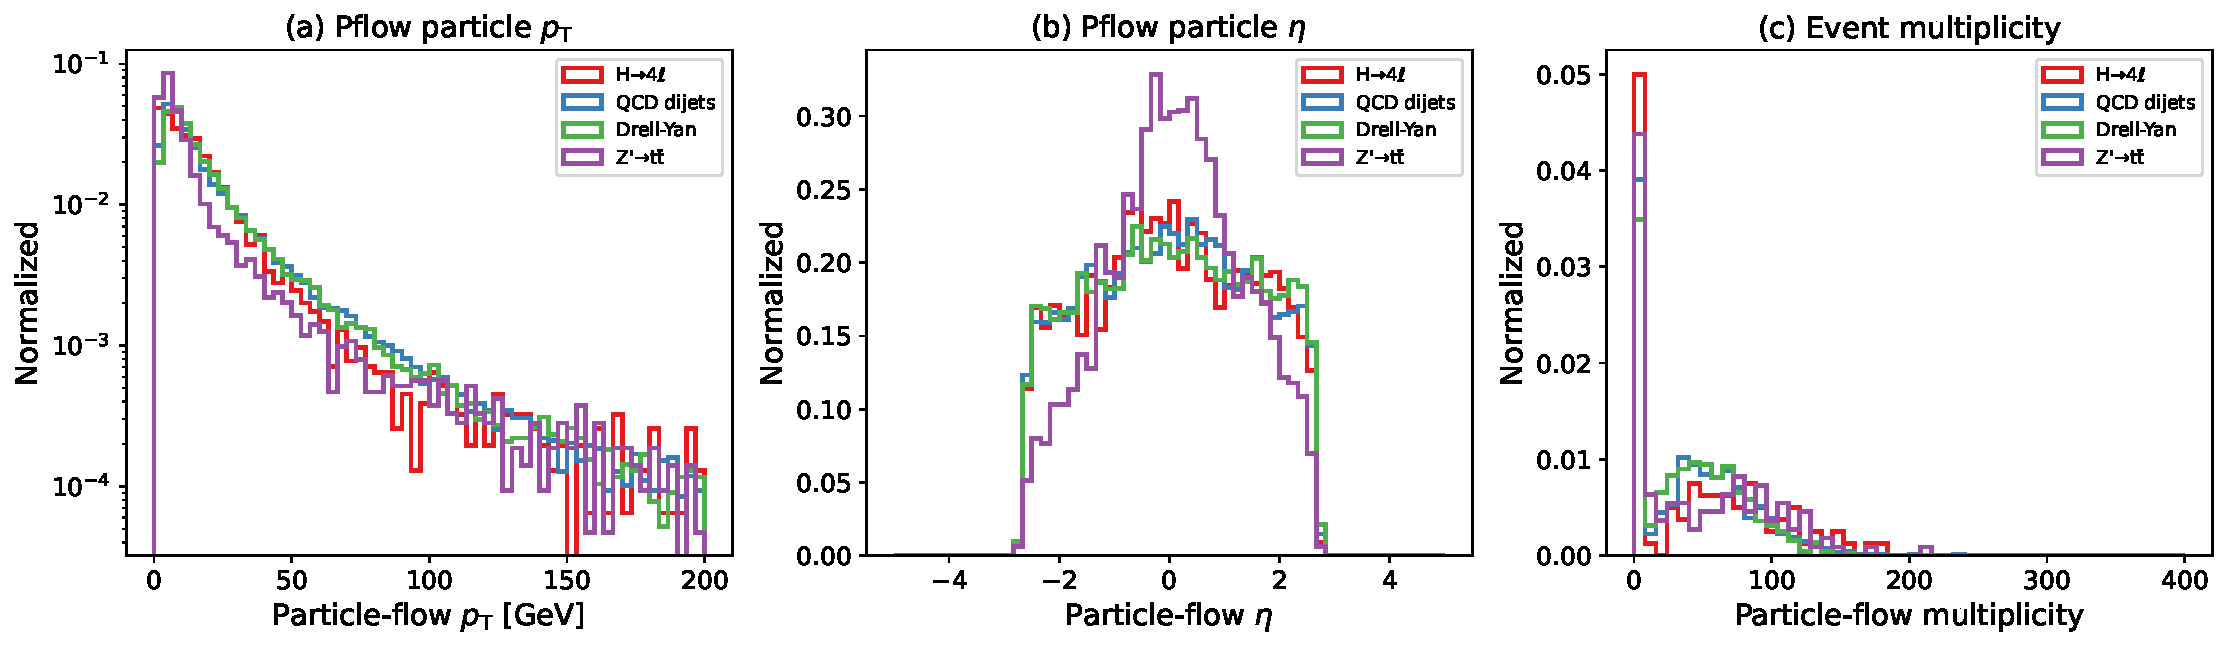
\includegraphics[width=\textwidth]{figures/kinematic_distributions_4proc.pdf}
\caption{Particle-flow kinematic distributions across four physics processes
  (including BSM $Z' \to t\bar{t}$).
  (a) Transverse momentum $p_\mathrm{T}$ in log scale,
  (b) pseudorapidity $\eta$,
  (c) particle-flow multiplicity per event. All distributions are normalised to
  unit area.}
\label{fig:kinematics}
\end{figure}

\subsection{Event-Level Quantities}

Figure~\ref{fig:eventlevel} shows the event-level quantities computed from the
Parnassus output: the scalar sum of transverse momenta $H_\mathrm{T}$, the
missing transverse energy $E_\mathrm{T}^\mathrm{miss}$, and the particle class
fractions. QCD dijets produce the hardest $H_\mathrm{T}$ spectrum as expected,
while all three processes show similar particle class compositions, dominated
by charged hadrons.

\begin{figure}[H]
\centering
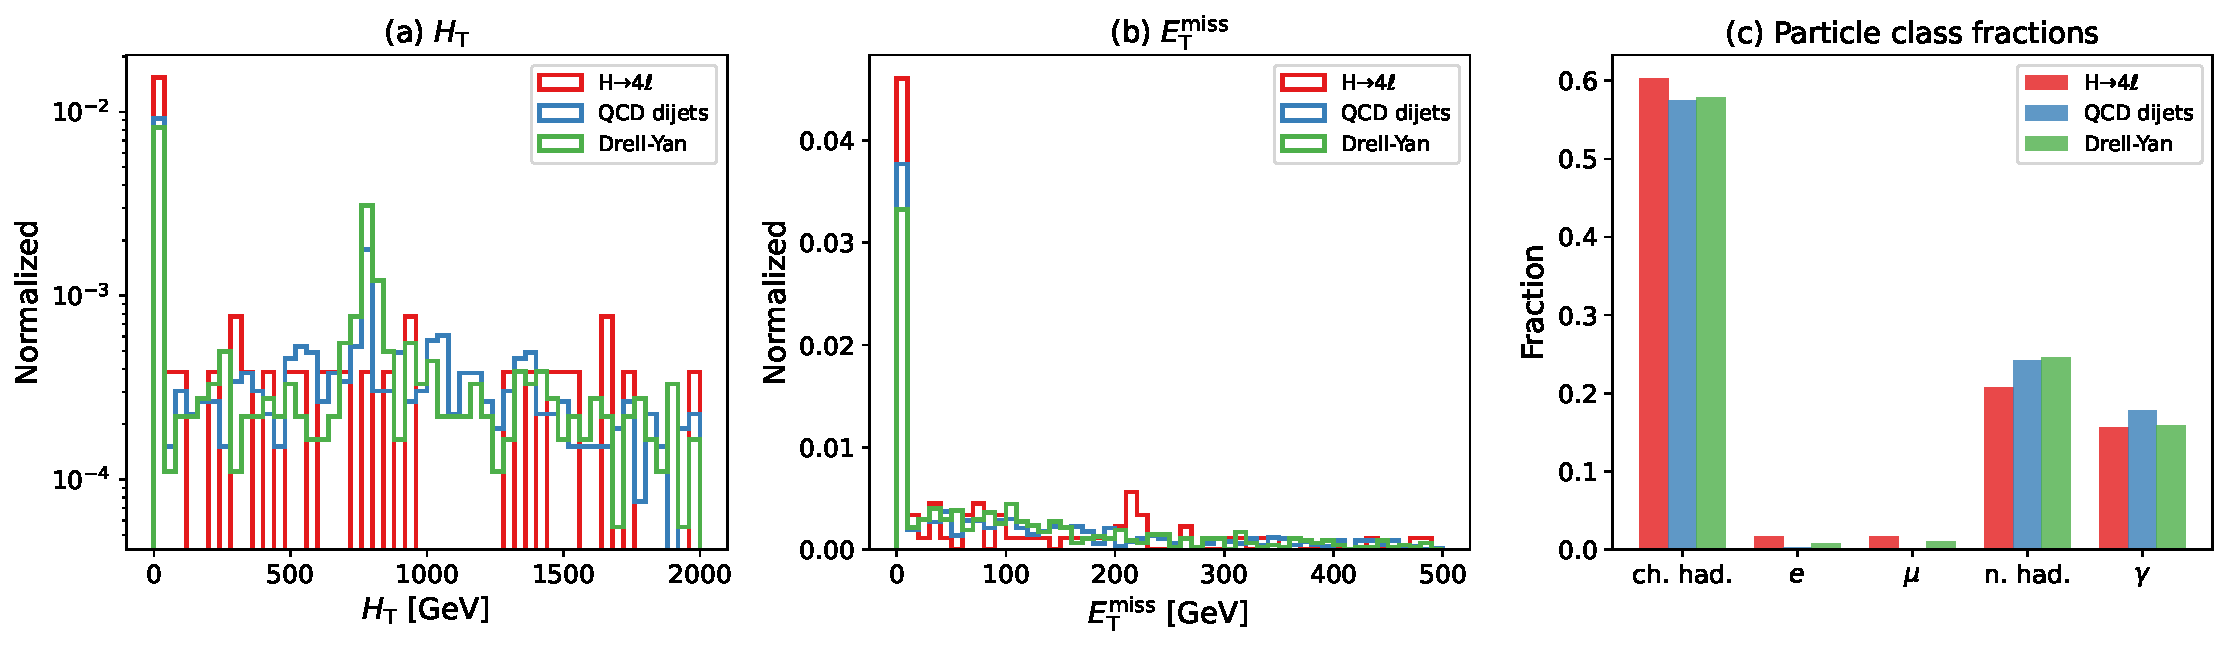
\includegraphics[width=\textwidth]{figures/event_level_distributions.pdf}
\caption{Event-level distributions.
  (a) $H_\mathrm{T}$ (scalar $p_\mathrm{T}$ sum),
  (b) $E_\mathrm{T}^\mathrm{miss}$,
  (c) particle class fractions per process. Charged hadrons dominate at
  ${\sim}58\%$, followed by neutral hadrons and photons.}
\label{fig:eventlevel}
\end{figure}

\subsection{Jet Distributions}

Figure~\ref{fig:jets} shows the reconstructed jet kinematics from the anti-$k_t$
algorithm with $R = 0.5$. The jet $p_\mathrm{T}$ spectra reflect the underlying
hard-scatter energy scale of each process, while the $\eta$ distributions are
broadly consistent across processes. The $Z' \to t\bar{t}$ process shows a
harder jet $p_\mathrm{T}$ spectrum due to the boosted top quarks from the heavy
resonance decay.

\begin{figure}[H]
\centering
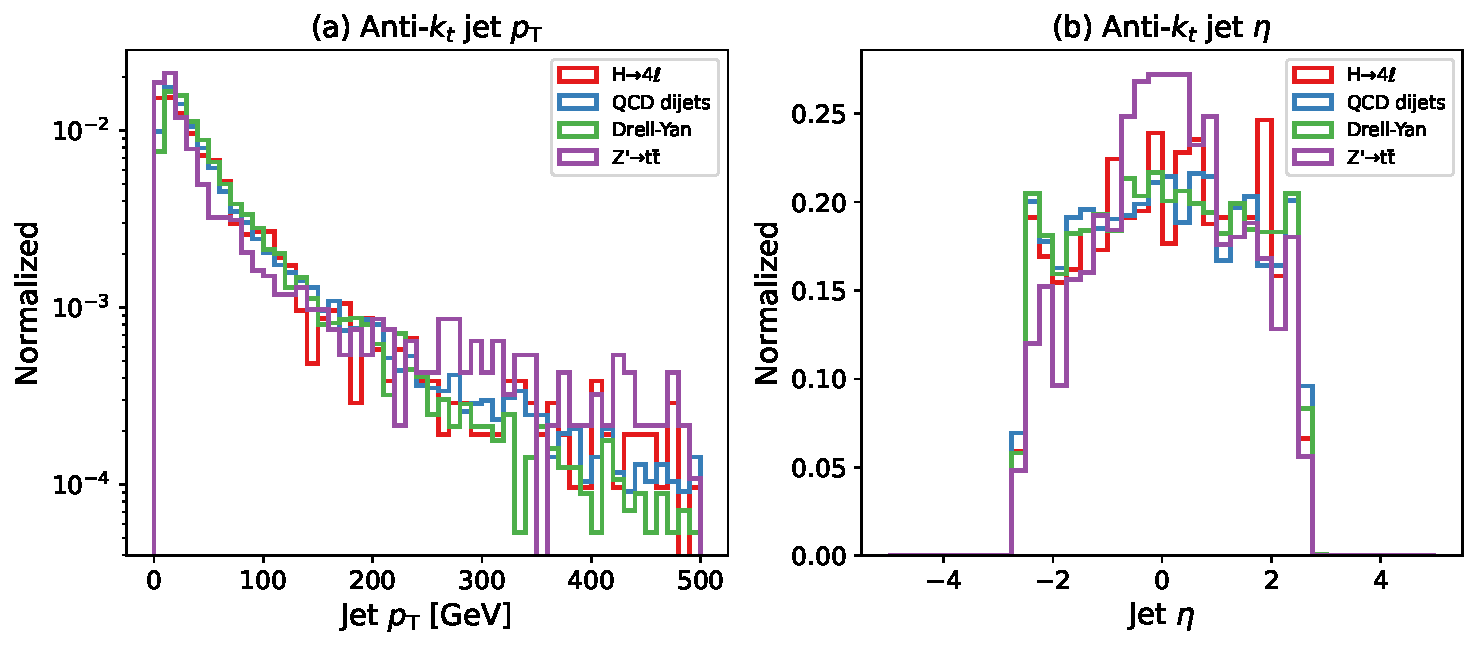
\includegraphics[width=\textwidth]{figures/jet_distributions_4proc.pdf}
\caption{Reconstructed jet distributions (anti-$k_t$, $R = 0.5$,
  $p_\mathrm{T}^\mathrm{min} = 10$\,GeV) across four processes including BSM.
  (a) Jet $p_\mathrm{T}$ in log scale,
  (b) jet pseudorapidity $\eta$.}
\label{fig:jets}
\end{figure}

\subsection{Event Displays}

The following event displays visualise individual events from each physics process
in the $\eta$--$\phi$ plane, providing an intuitive picture of how Parnassus
transforms truth-level particles into detector-level particle-flow objects.

\subsubsection{$H \to ZZ \to 4\ell$}

Figure~\ref{fig:display_h4l} shows a representative $H \to ZZ \to 4\ell$ event.
The truth-level particles (left) are mapped to pflow objects (right) with particle
identification indicated by colour and marker shape. Anti-$k_t$ jets are shown as
dashed circles.

\begin{figure}[H]
\centering
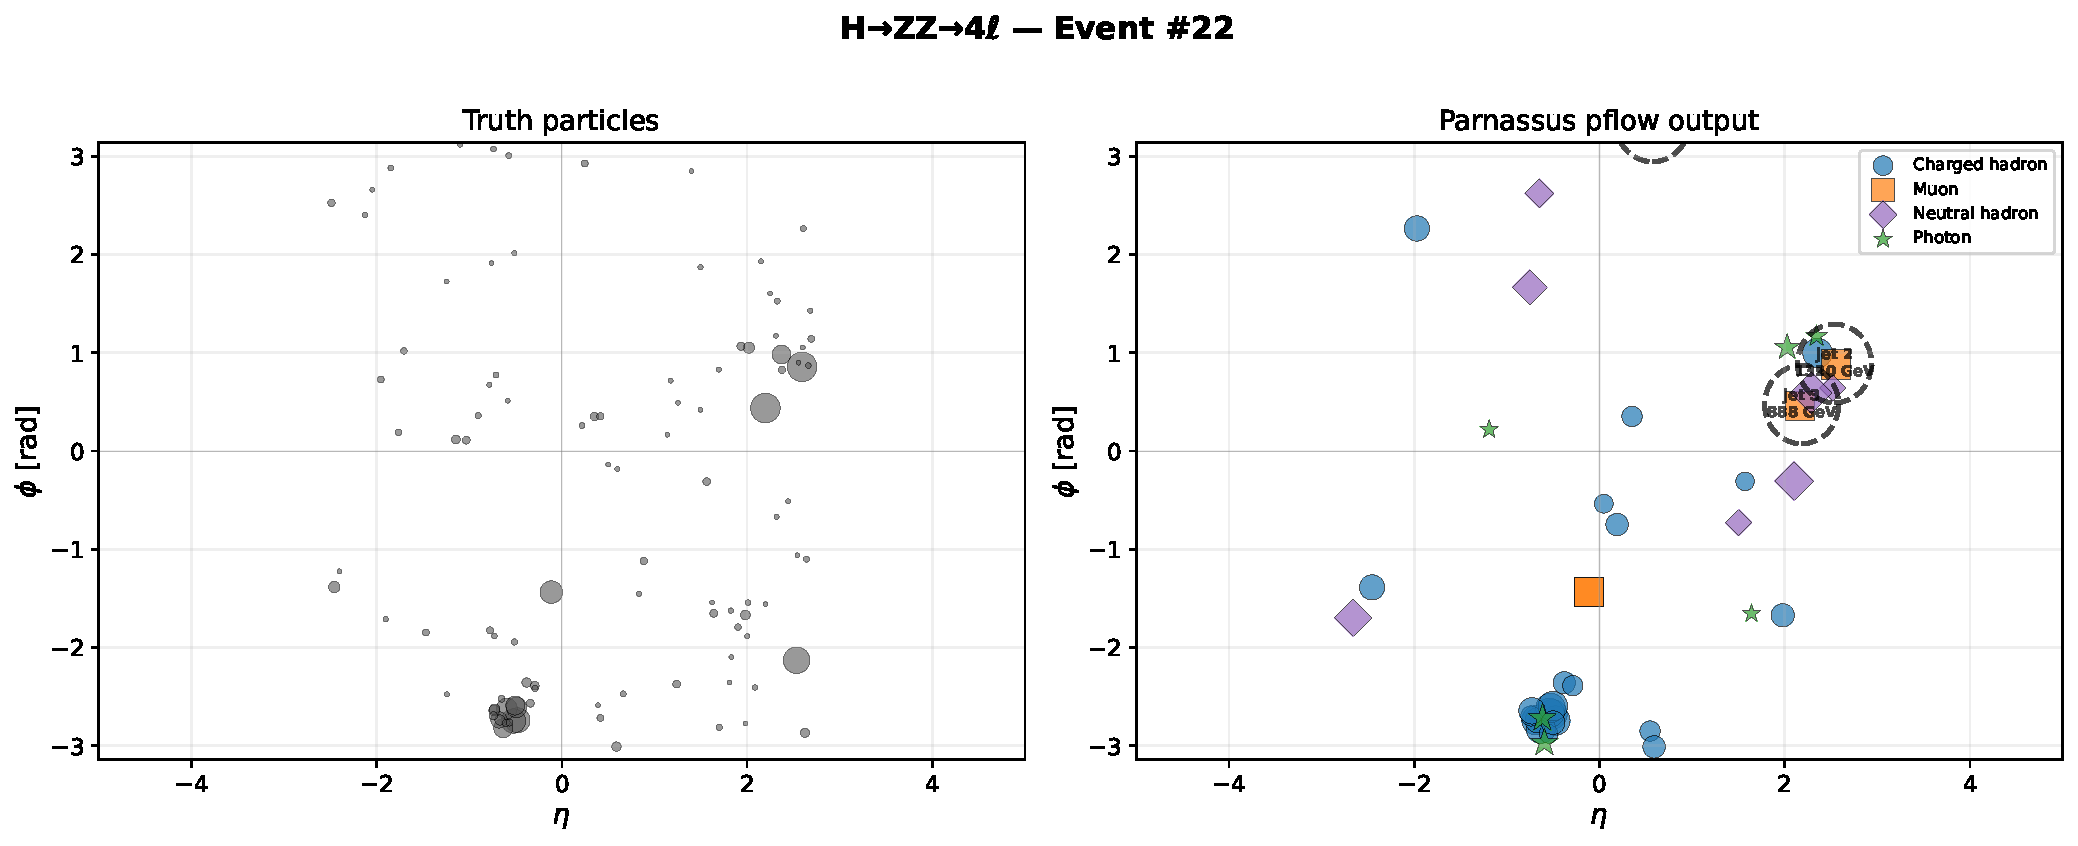
\includegraphics[width=\textwidth]{figures/event_display_h4l.pdf}
\caption{Event display for $H \to ZZ \to 4\ell$: truth particles (left) and
  Parnassus pflow output (right) in the $\eta$--$\phi$ plane. Marker size scales
  with $p_\mathrm{T}$; dashed circles indicate anti-$k_t$ jets ($R = 0.5$).
  Particle classes: charged hadrons (blue circles), electrons (red triangles),
  muons (orange squares), neutral hadrons (purple diamonds), photons (green stars).}
\label{fig:display_h4l}
\end{figure}

\subsubsection{QCD Dijets}

Figure~\ref{fig:display_qcd} shows a QCD dijet event with its characteristic
back-to-back jet topology clearly visible in both truth and pflow representations.

\begin{figure}[H]
\centering
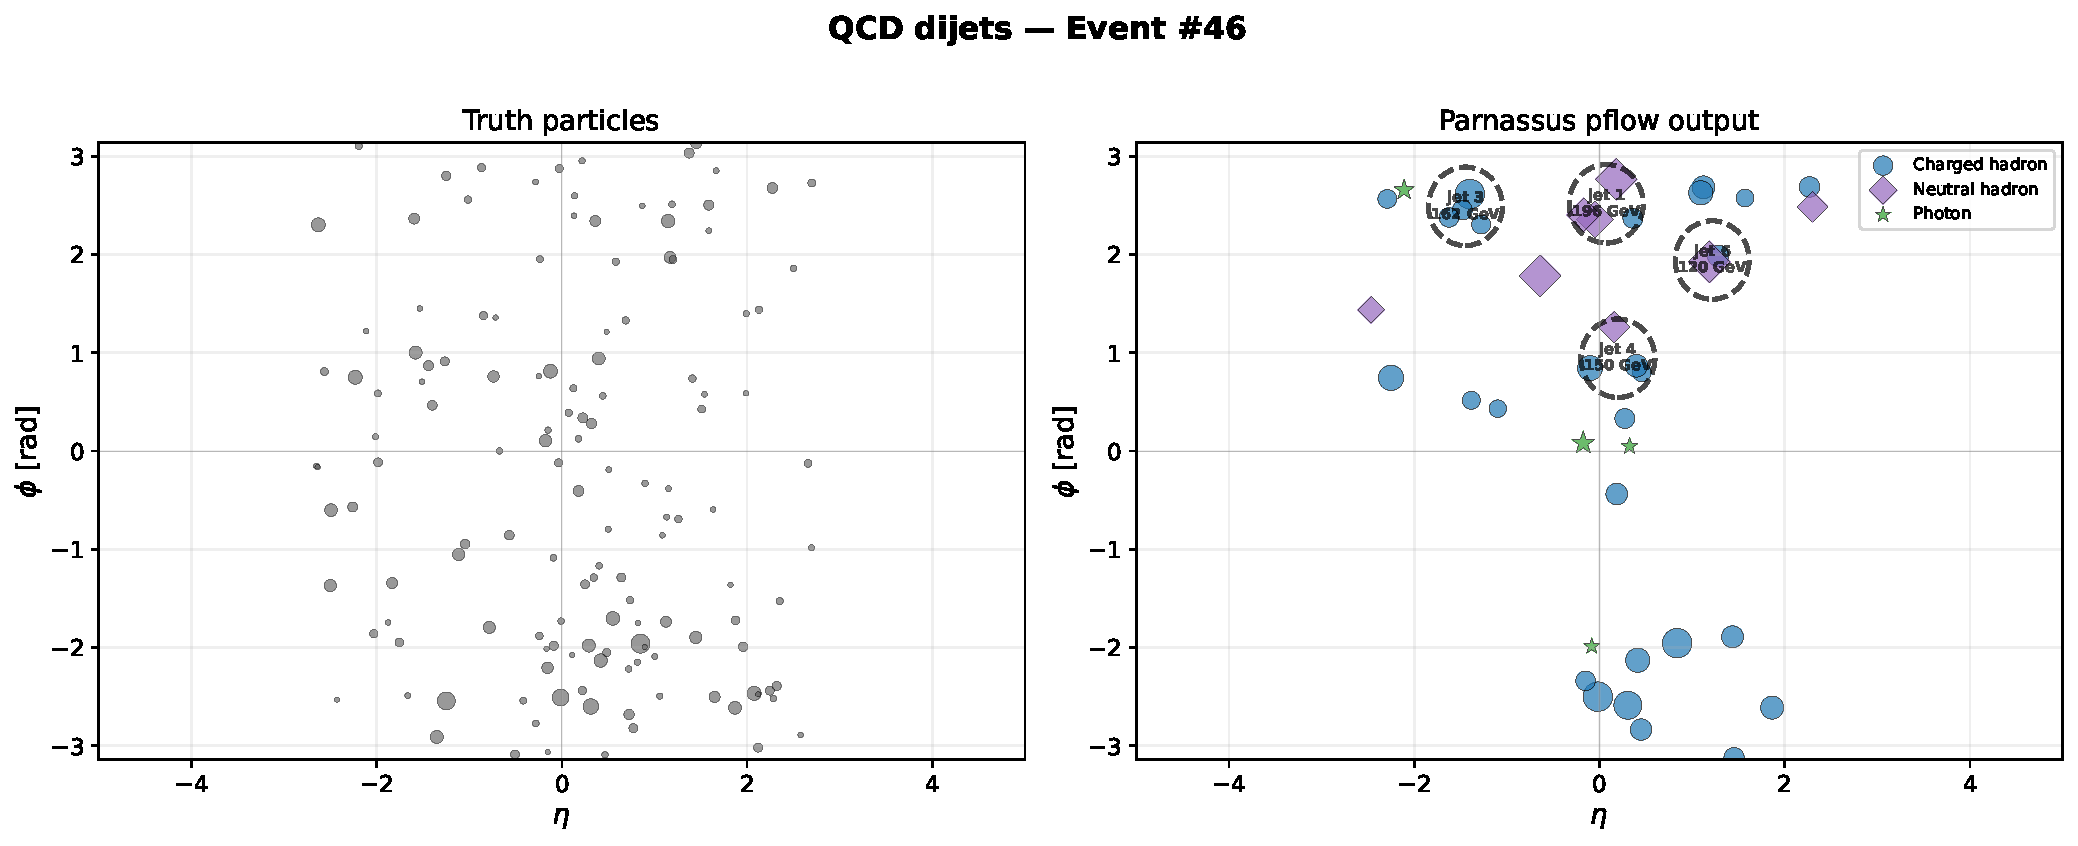
\includegraphics[width=\textwidth]{figures/event_display_qcd.pdf}
\caption{Event display for QCD dijets: truth particles (left) and Parnassus pflow
  output (right). The back-to-back jet structure from the hard QCD scatter is
  reproduced in the pflow output.}
\label{fig:display_qcd}
\end{figure}

\subsubsection{Drell--Yan}

Figure~\ref{fig:display_dy} shows a Drell--Yan $Z/\gamma^* \to \ell\ell$ event
where the leptonic decay products are visible alongside the underlying event activity.

\begin{figure}[H]
\centering
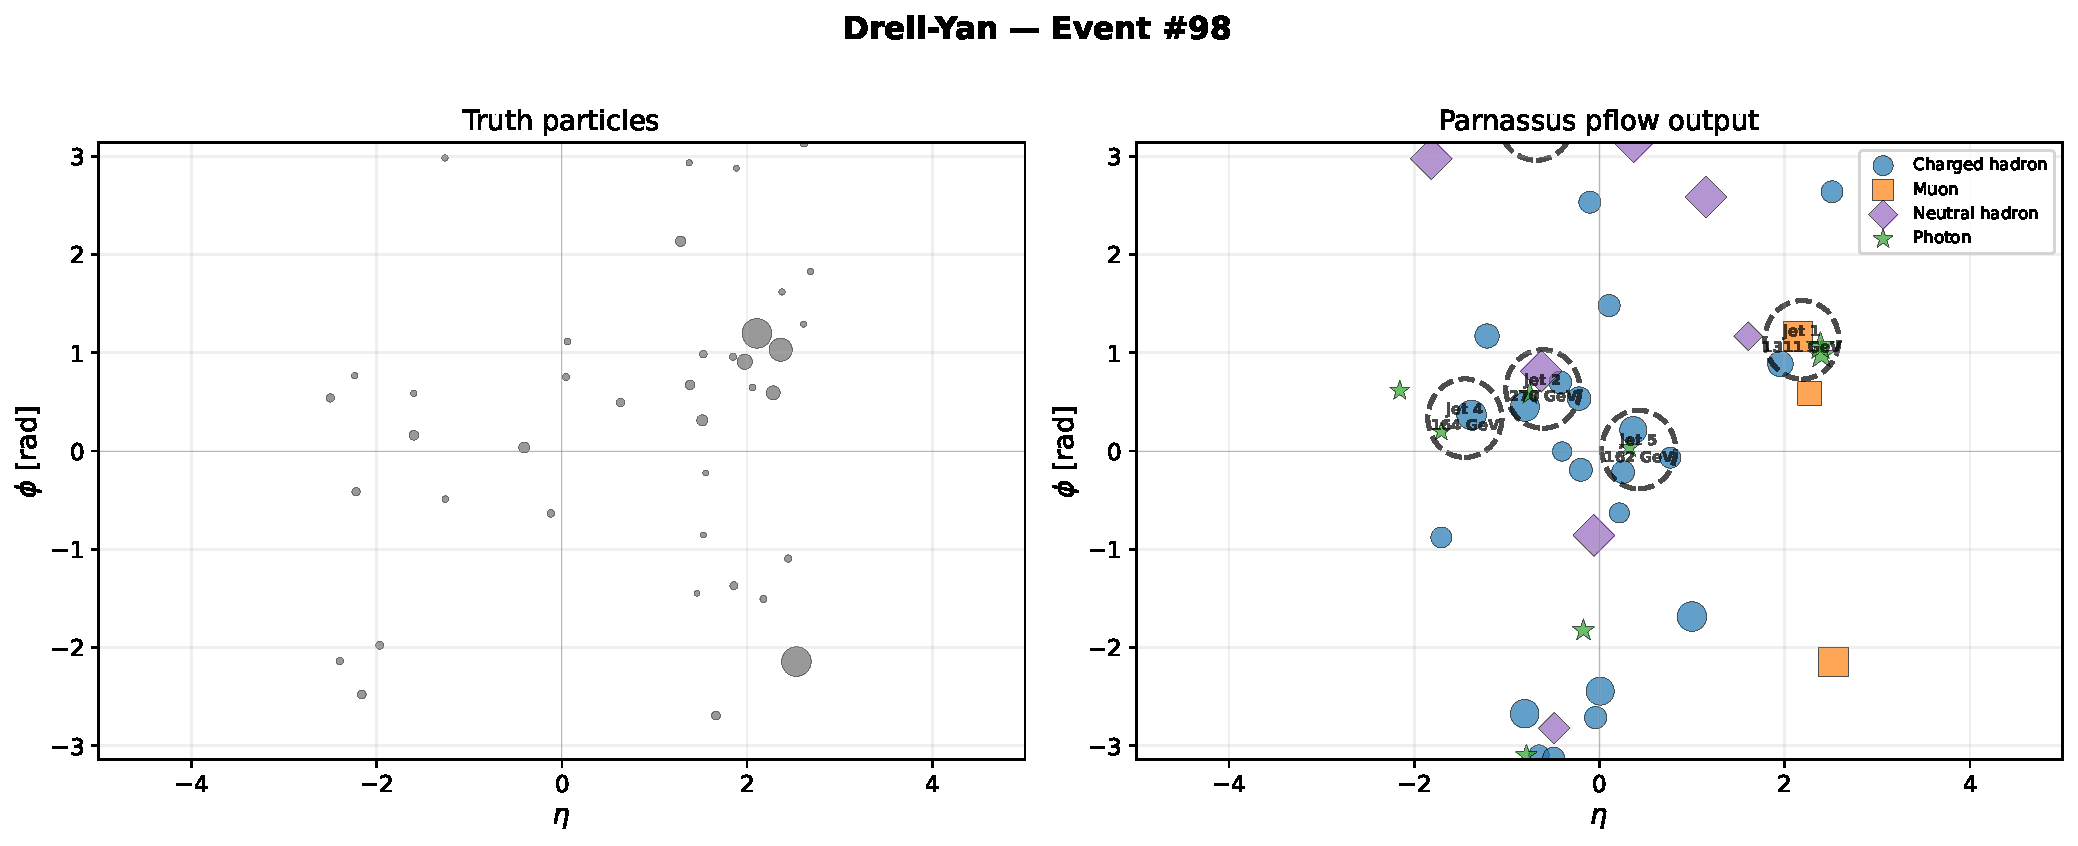
\includegraphics[width=\textwidth]{figures/event_display_dy.pdf}
\caption{Event display for Drell--Yan $Z/\gamma^* \to \ell\ell$: truth particles
  (left) and Parnassus pflow output (right).}
\label{fig:display_dy}
\end{figure}

\subsubsection{BSM: $Z' \to t\bar{t}$ (1\,TeV)}

Figure~\ref{fig:display_zprime} shows a BSM $Z' \to t\bar{t}$ event. The high
truth-particle multiplicity from the boosted top decays is clearly visible on
the left. The pflow output on the right shows the reconstructed event with
leptons, hadrons, and photons from the top decay products.

\begin{figure}[H]
\centering
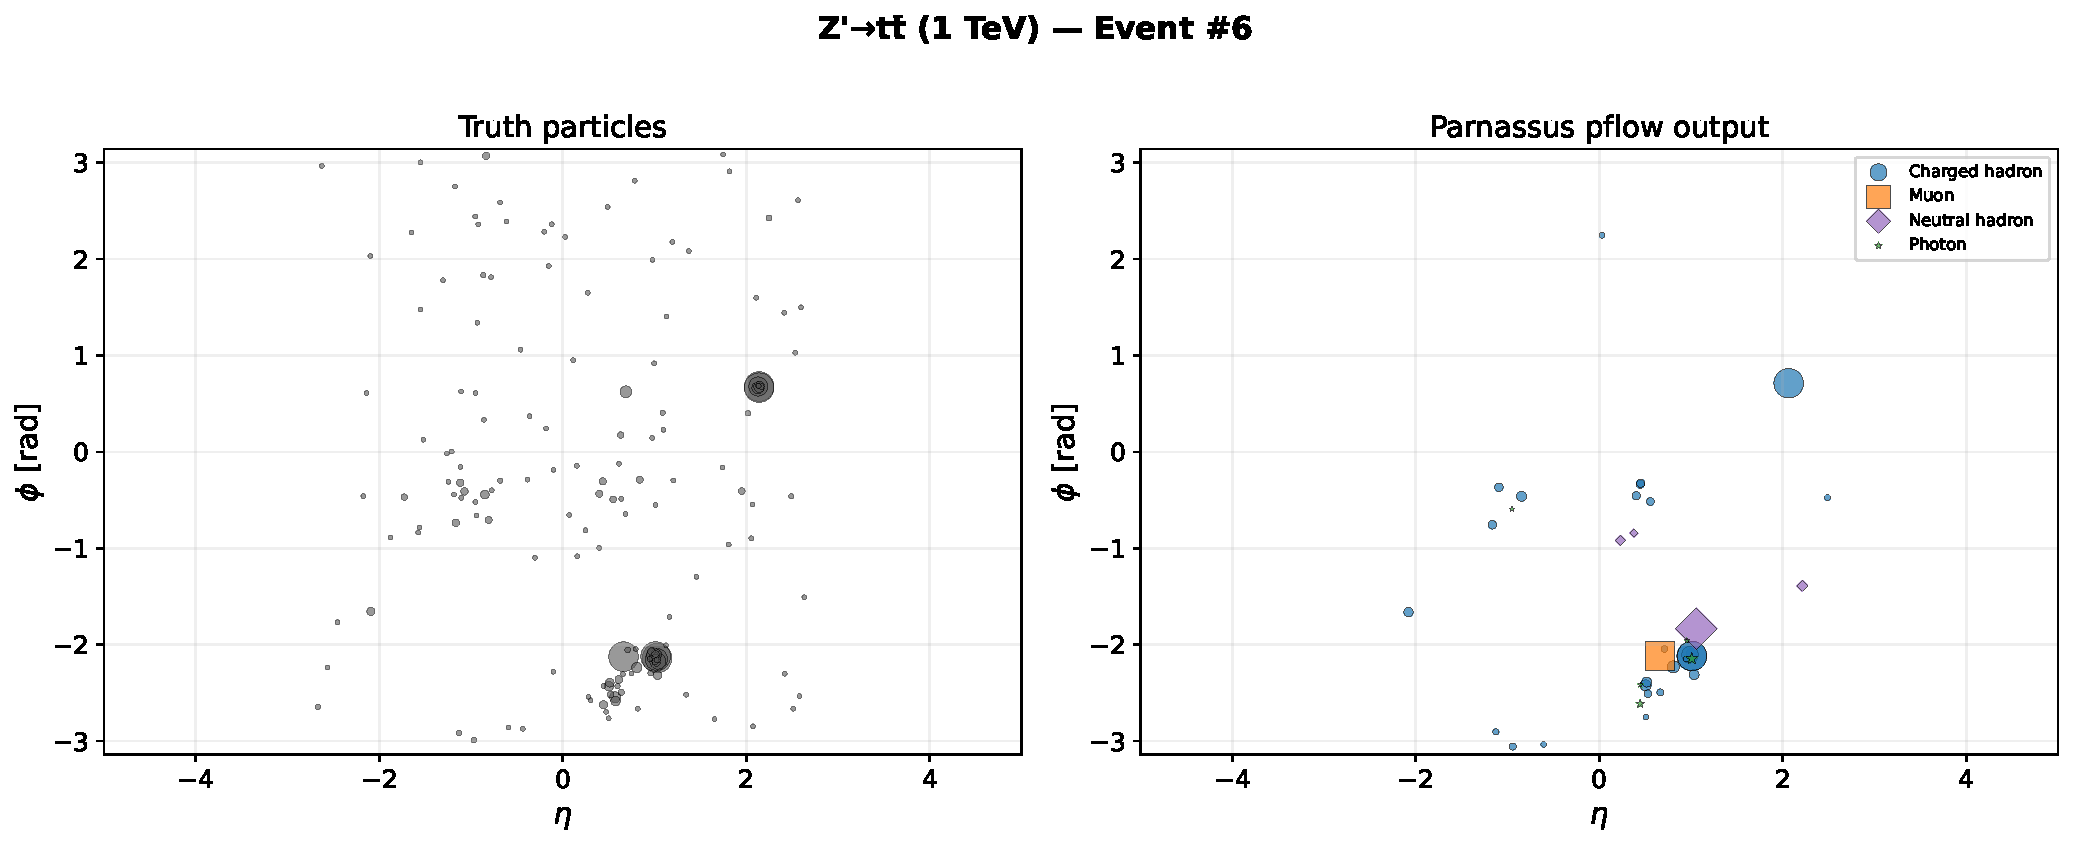
\includegraphics[width=\textwidth]{figures/event_display_zprime.pdf}
\caption{Event display for BSM $Z' \to t\bar{t}$ (1\,TeV): truth particles (left) and
  Parnassus pflow output (right). This process was not present in the training data,
  demonstrating the model's process-agnostic generalization.}
\label{fig:display_zprime}
\end{figure}

\subsubsection{Energy Flow (Lego) Plots}

Figures~\ref{fig:lego_h4l}--\ref{fig:lego_dy} show the $p_\mathrm{T}$-weighted
energy flow in the $\eta$--$\phi$ plane as 3D lego plots, comparing truth-level
and pflow distributions for each process.

\begin{figure}[H]
\centering
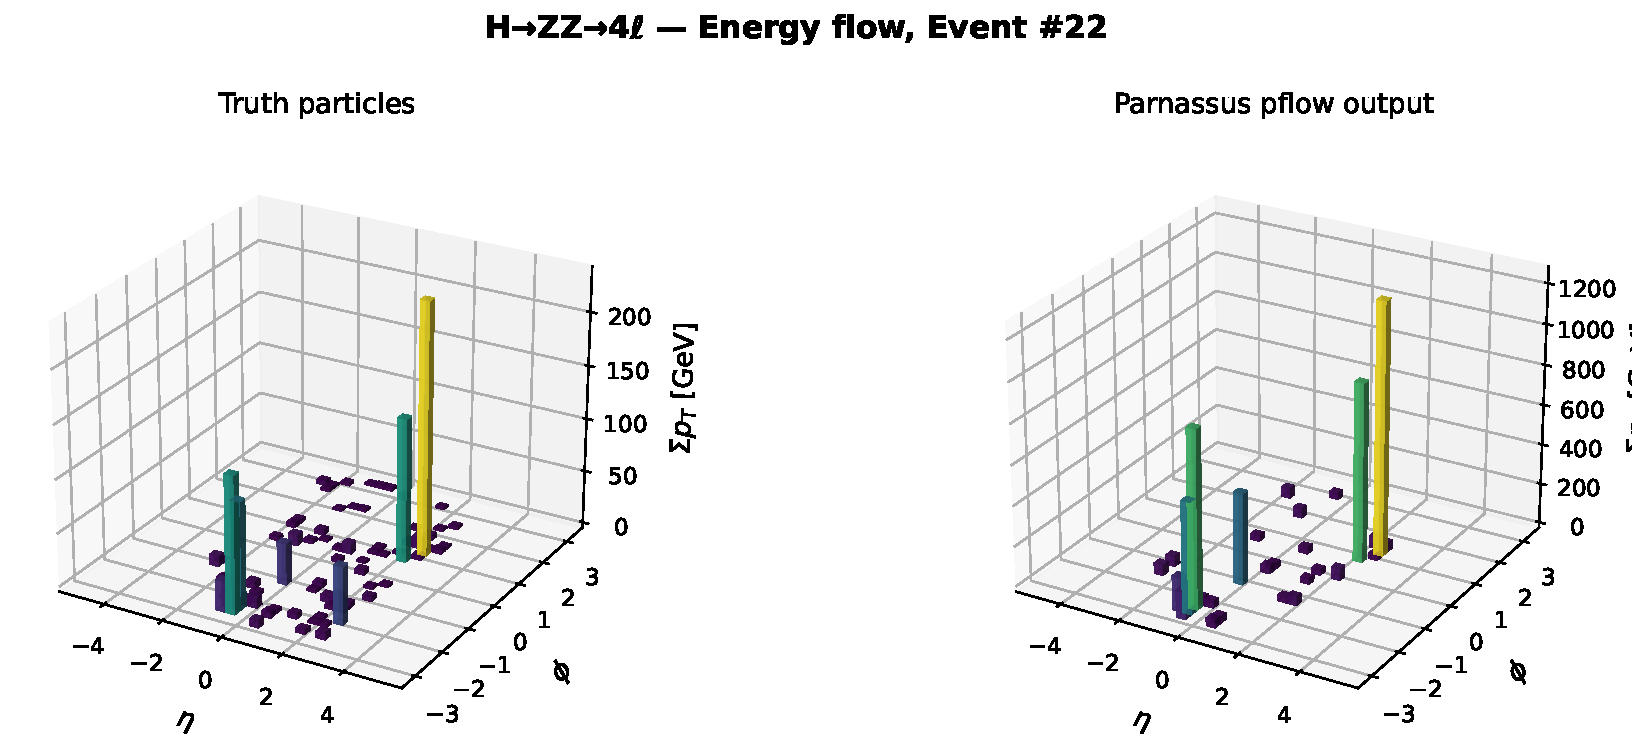
\includegraphics[width=\textwidth]{figures/event_display_h4l_lego.pdf}
\caption{Energy flow lego plot for $H \to ZZ \to 4\ell$: truth (left) vs.\
  pflow (right). Each bin shows the scalar $p_\mathrm{T}$ sum.}
\label{fig:lego_h4l}
\end{figure}

\begin{figure}[H]
\centering
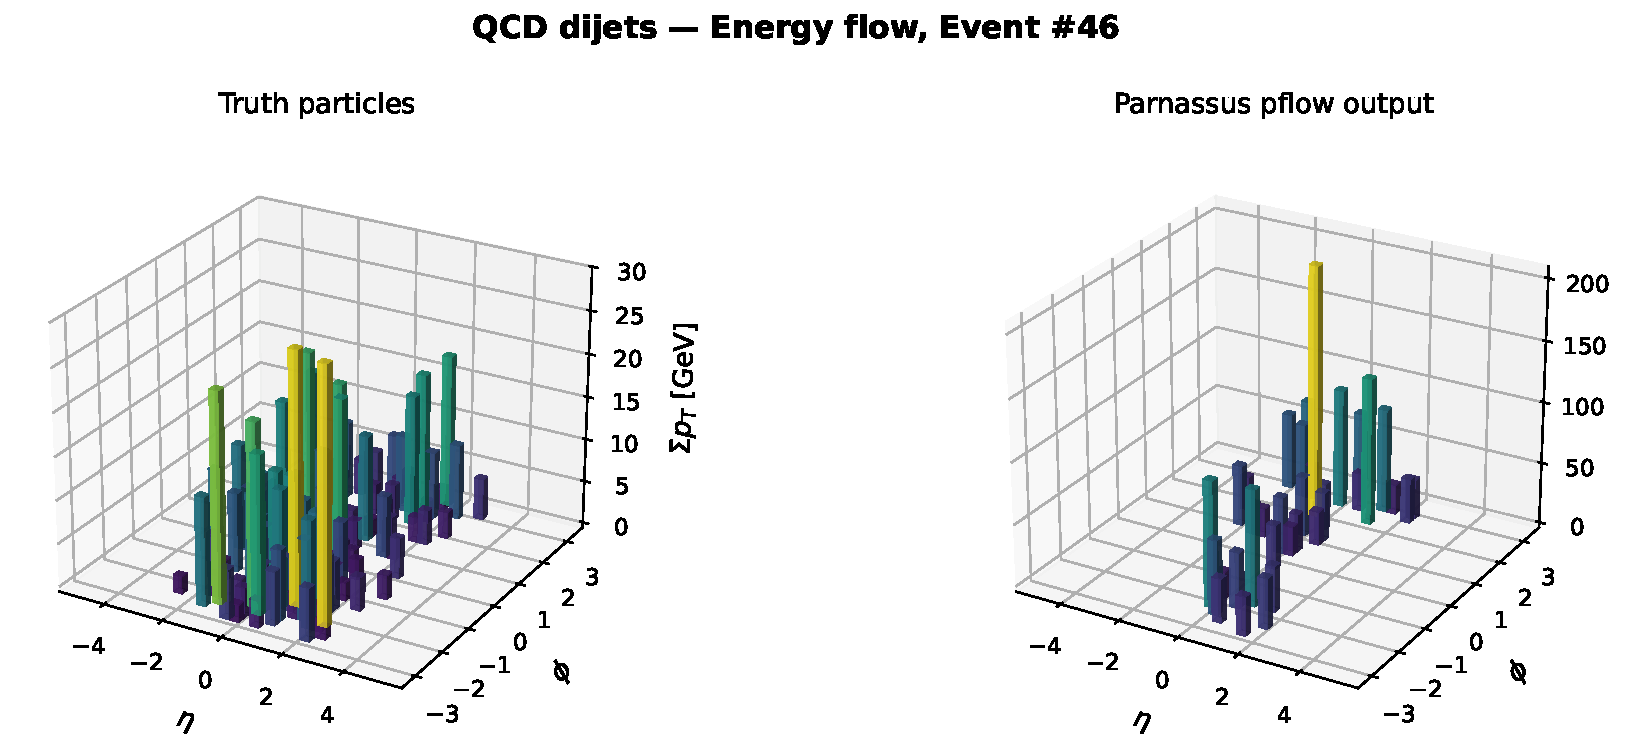
\includegraphics[width=\textwidth]{figures/event_display_qcd_lego.pdf}
\caption{Energy flow lego plot for QCD dijets: truth (left) vs.\ pflow (right).}
\label{fig:lego_qcd}
\end{figure}

\begin{figure}[H]
\centering
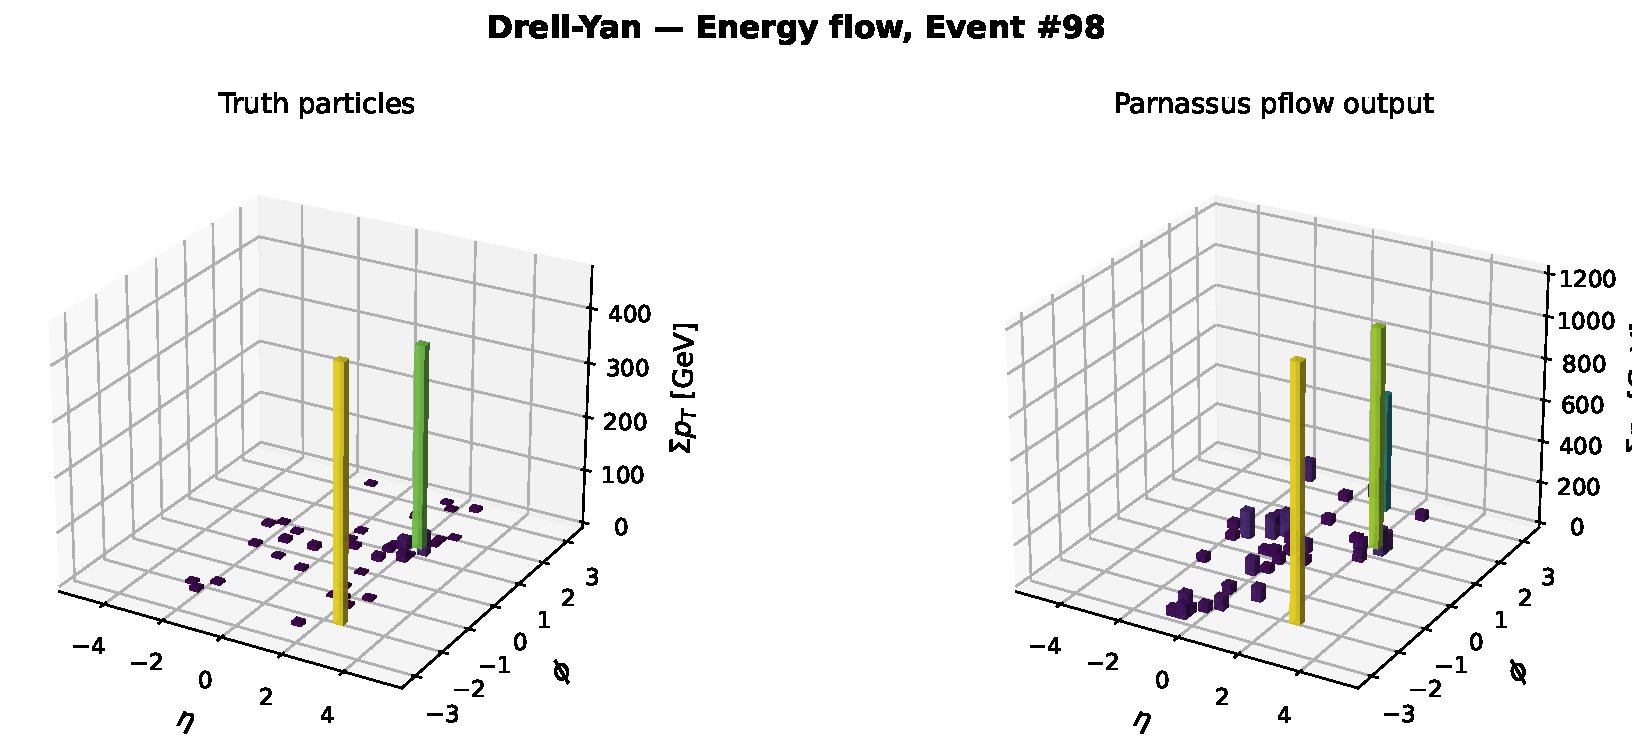
\includegraphics[width=\textwidth]{figures/event_display_dy_lego.pdf}
\caption{Energy flow lego plot for Drell--Yan: truth (left) vs.\ pflow (right).}
\label{fig:lego_dy}
\end{figure}

\begin{figure}[H]
\centering
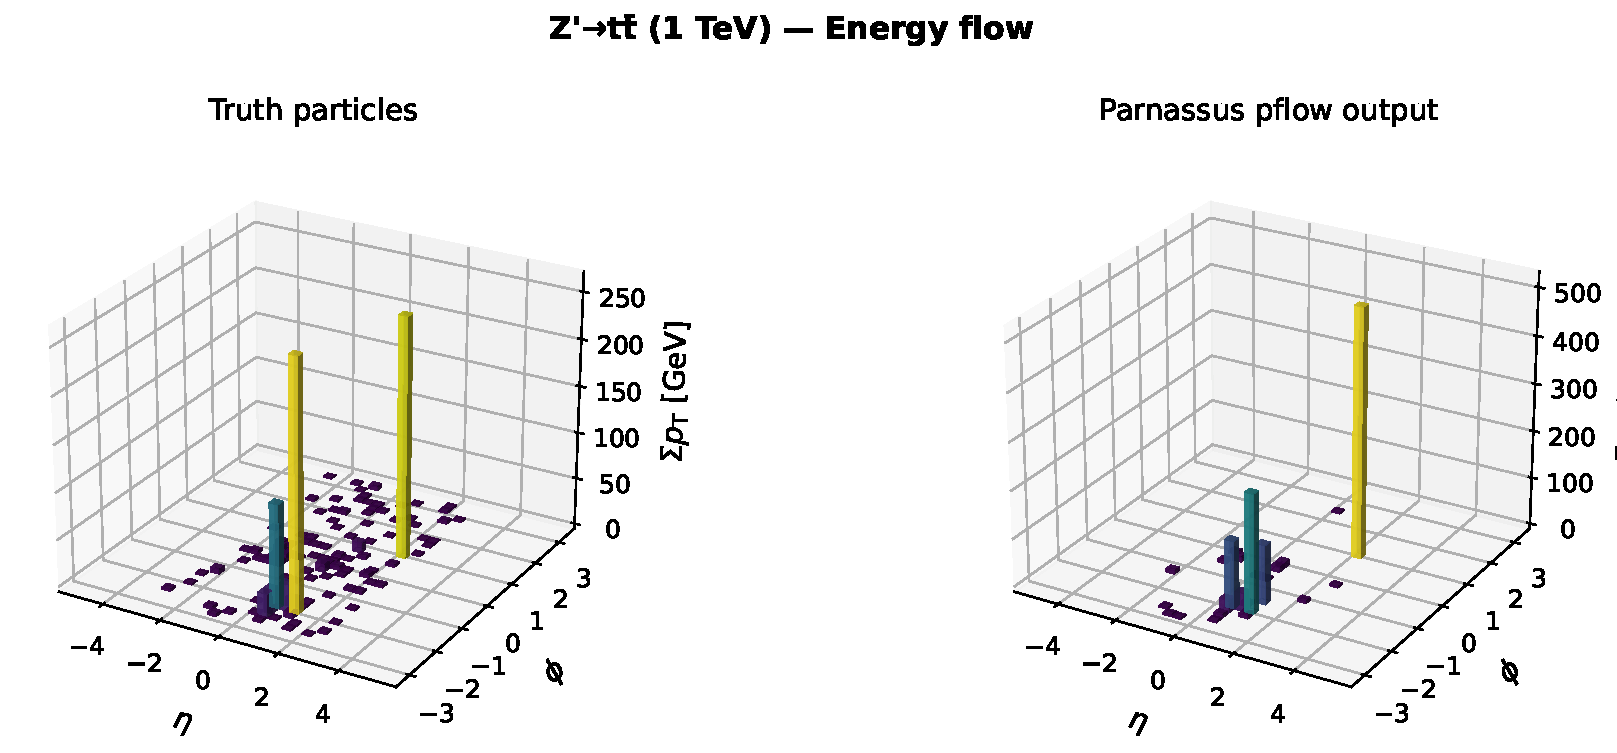
\includegraphics[width=\textwidth]{figures/event_display_zprime_lego.pdf}
\caption{Energy flow lego plot for BSM $Z' \to t\bar{t}$ (1\,TeV): truth (left)
  vs.\ pflow (right). The high energy deposit from boosted top decays is visible.}
\label{fig:lego_zprime}
\end{figure}

\subsubsection{Process Comparison}

Figure~\ref{fig:process_comparison} provides a side-by-side comparison of single
events from all four processes, highlighting the different event topologies
and demonstrating the model's ability to handle diverse physics signatures,
including BSM signals not present in the training data.

\begin{figure}[H]
\centering
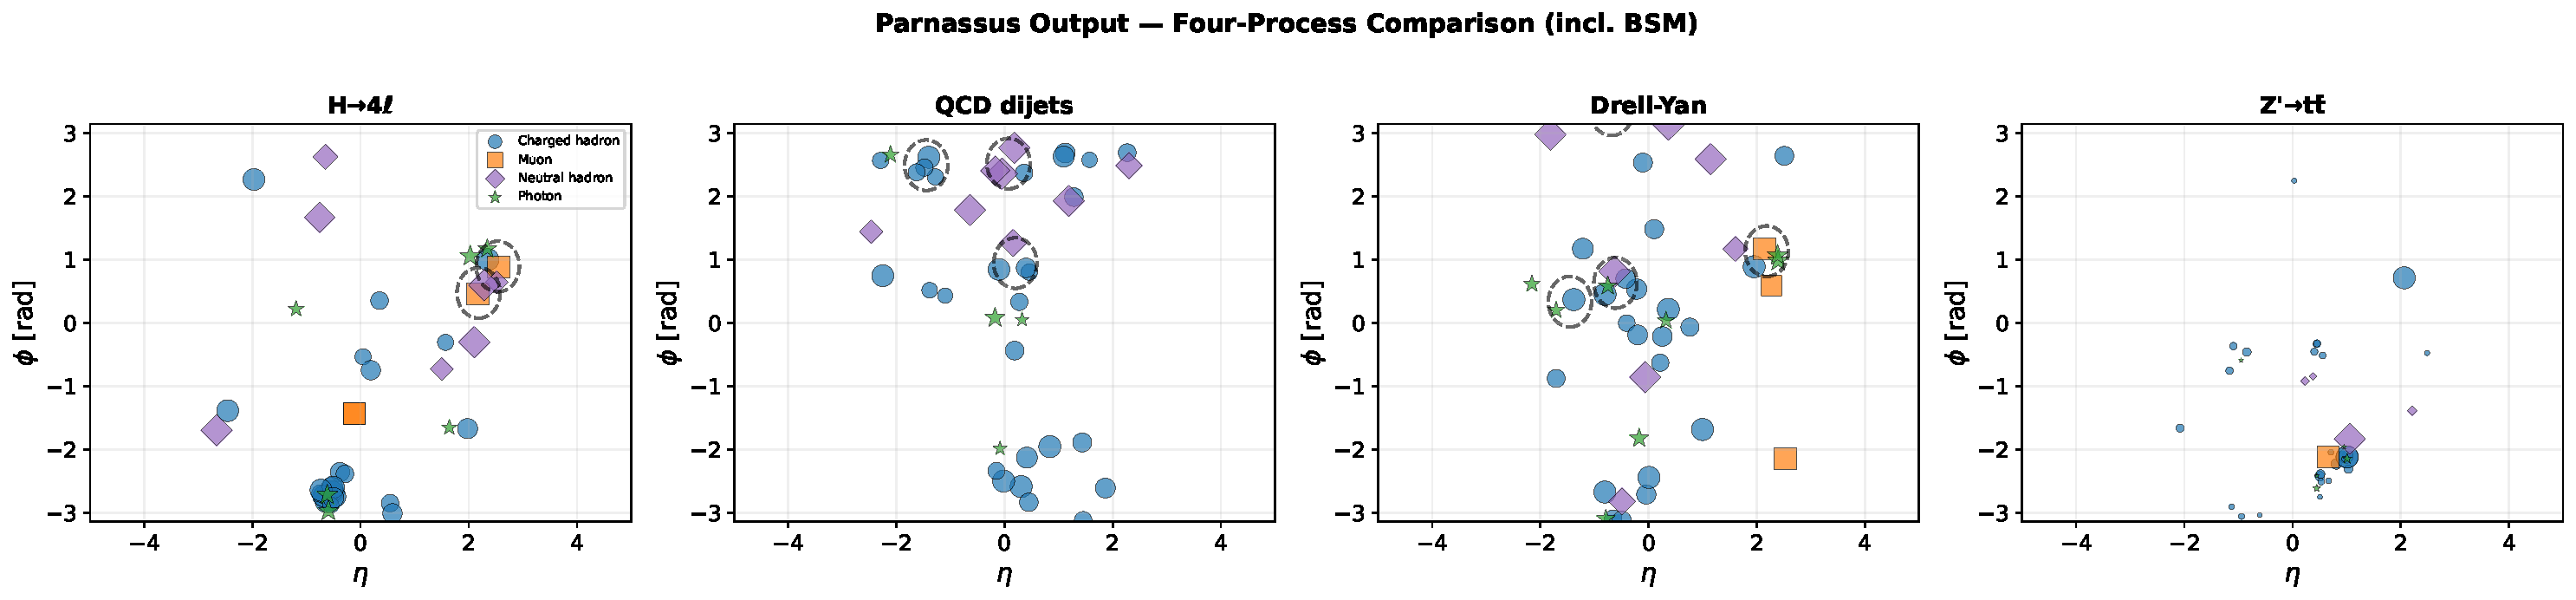
\includegraphics[width=\textwidth]{figures/process_comparison_4proc.pdf}
\caption{Side-by-side comparison of Parnassus pflow output for four physics
  processes including BSM. Each panel shows one representative event in
  $\eta$--$\phi$ with particle classes colour-coded and anti-$k_t$ jets
  overlaid as dashed circles.
  The distinct event topologies --- low-multiplicity leptonic ($H \to 4\ell$),
  hadronic dijet (QCD), electroweak (Drell--Yan), and BSM heavy resonance
  ($Z' \to t\bar{t}$) --- are all produced by the same pre-trained model.}
\label{fig:process_comparison}
\end{figure}

\subsection{Aggregate Statistics Across Processes}

Table~\ref{tab:aggregate} compares the aggregate statistics across the three processes.
The model adapts to different truth-particle multiplicities and kinematics.

\begin{table}[H]
\centering
\caption{Aggregate statistics across four physics processes (mean $\pm$ std).}
\label{tab:aggregate}
\begin{tabular}{@{}lrrrr@{}}
\toprule
\textbf{Quantity}
  & \textbf{$H{\to}4\ell$}
  & \textbf{QCD dijet}
  & \textbf{Drell--Yan}
  & \textbf{$Z'{\to}t\bar{t}$} \\
  & \textbf{(100\,evt)}
  & \textbf{(832\,evt)}
  & \textbf{(555\,evt)}
  & \textbf{(137\,evt)} \\
\midrule
Truth particles/event  & $96.4 \pm 46.4$   & $107.1 \pm 45.9$  & $76.1 \pm 39.3$ & $169.0 \pm 49.4$ \\
Pflow particles/event  & $47.4 \pm 48.5$   & $43.2 \pm 39.4$   & $42.3 \pm 36.5$ & $47.6 \pm 47.5$ \\
Truth $H_\mathrm{T}$ (GeV) & $793.6 \pm 171.2$ & $775.1 \pm 166.8$ & $786.4 \pm 137.4$ & --- \\
Pflow $H_\mathrm{T}$ (GeV) & $1375 \pm 1614$   & $1262 \pm 1680$   & $1187 \pm 1486$ & $1219 \pm 1517$ \\
\bottomrule
\end{tabular}
\end{table}

\noindent
The $Z' \to t\bar{t}$ process shows significantly higher truth-particle multiplicity
($169 \pm 49$) compared to the SM processes, reflecting the busy final state from
top quark decays at a 1\,TeV resonance mass. Despite this, the pflow output
multiplicity ($47.6 \pm 47.5$) is comparable to the SM processes, and the model
produces physically reasonable output without any process-specific tuning.

\subsection{Per-Event Output}

Table~\ref{tab:perevt} shows the first 10 events from each process to illustrate
event-by-event variation.

\begin{table}[H]
\centering
\caption{Per-event summary: first 10 events from each process (50 diffusion steps).}
\label{tab:perevt}
\small
\begin{tabular}{@{}clrrrr@{}}
\toprule
\textbf{Process} & \textbf{Evt} & \textbf{$n_\mathrm{truth}$} & \textbf{$n_\mathrm{pflow}$}
  & \textbf{Truth $H_\mathrm{T}$} & \textbf{Pflow $H_\mathrm{T}$} \\
\midrule
\multirow{10}{*}{\rotatebox{90}{\small$H{\to}4\ell$}}
  & 0  & 105 &  86 &  723 & 2165 \\
  & 1  & 143 &  63 &  789 & 2431 \\
  & 2  &  26 &   0 & 1189 &    0 \\
  & 3  & 126 &   0 &  832 &    0 \\
  & 4  & 174 &  11 &  805 &   54 \\
  & 5  &  60 & 177 &  843 &  684 \\
  & 6  & 132 &  47 &  820 & 2550 \\
  & 7  &  71 &  64 & 1150 &  439 \\
  & 8  &  37 &   0 &  638 &    0 \\
  & 9  &  89 & 116 &  831 &  952 \\
\midrule
\multirow{10}{*}{\rotatebox{90}{\small QCD dijet}}
  & 0  & 110 & 109 &  717 & 1564 \\
  & 1  &  38 &   0 &  966 &    0 \\
  & 2  & 102 &  95 &  693 &  992 \\
  & 3  & 230 &  24 &  817 &   42 \\
  & 4  &  81 &  69 &  819 & 4175 \\
  & 5  &  61 & 111 &  537 &  462 \\
  & 6  & 106 &   0 &  694 &    0 \\
  & 7  & 109 &   0 &  778 &    0 \\
  & 8  &  92 &   0 &  945 &    0 \\
  & 9  &  70 &  54 &  780 & 1860 \\
\midrule
\multirow{10}{*}{\rotatebox{90}{\small Drell--Yan}}
  & 0  & 114 &  14 &  856 & 3822 \\
  & 1  &  83 &  99 &  738 & 1968 \\
  & 2  &  16 &  36 &  498 &  817 \\
  & 3  &  90 &   0 &  783 &    0 \\
  & 4  &  48 &  59 &  665 &  681 \\
  & 5  & 101 &  46 &  772 &  735 \\
  & 6  & 146 & 131 &  803 &  863 \\
  & 7  &  60 &  36 &  848 & 1763 \\
  & 8  &  89 &  66 &  833 & 5109 \\
  & 9  &  61 &  48 &  978 & 1744 \\
\bottomrule
\end{tabular}
\end{table}

\subsection{Particle Class Distribution}

Table~\ref{tab:classdist} compares the particle class composition between truth
and pflow particles for all three processes. The class fractions are broadly
consistent: charged hadrons dominate at ${\sim}55$--$60\%$, photons decrease
from ${\sim}31\%$ (truth) to ${\sim}16\%$ (pflow), and neutral hadrons increase
from ${\sim}7$--$10\%$ to ${\sim}21$--$25\%$.

\begin{table}[H]
\centering
\caption{Particle class distribution by process (truth $\to$ pflow percentages).}
\label{tab:classdist}
\begin{tabular}{@{}lrrrrrrrr@{}}
\toprule
& \multicolumn{2}{c}{\textbf{$H{\to}4\ell$}}
& \multicolumn{2}{c}{\textbf{QCD dijet}}
& \multicolumn{2}{c}{\textbf{Drell--Yan}}
& \multicolumn{2}{c}{\textbf{$Z'{\to}t\bar{t}$}} \\
\cmidrule(lr){2-3}\cmidrule(lr){4-5}\cmidrule(lr){6-7}\cmidrule(lr){8-9}
\textbf{Class} & \textbf{Tr.} & \textbf{Pf.}
  & \textbf{Tr.} & \textbf{Pf.}
  & \textbf{Tr.} & \textbf{Pf.}
  & \textbf{Tr.} & \textbf{Pf.} \\
\midrule
Ch.\ hadron & 54.8\% & 60.3\% & 59.7\% & 57.5\% & 60.4\% & 57.9\% & 55.5\% & 59.6\% \\
Electron    &  1.5\% &  1.6\% &  0.3\% &  0.3\% &  0.9\% &  0.7\% &  0.9\% &  0.9\% \\
Muon        &  1.7\% &  1.7\% &  0.1\% &  0.2\% &  0.8\% &  1.0\% &  0.5\% &  1.0\% \\
N.\ hadron  & 10.4\% & 20.8\% &  6.8\% & 24.2\% &  6.9\% & 24.6\% &  6.1\% & 16.5\% \\
Photon      & 31.6\% & 15.7\% & 33.1\% & 17.8\% & 30.9\% & 15.8\% & 37.0\% & 22.1\% \\
\midrule
Total       & 9\,644 & 4\,742 & 89\,119 & 35\,965 & 42\,243 & 23\,474 & 23\,158 & 6\,518 \\
\bottomrule
\end{tabular}
\end{table}

\subsection{Jet Reconstruction}

Table~\ref{tab:jets_table} summarises the jet reconstruction results using the
anti-$k_t$ algorithm with $R = 0.5$ across all three processes.

\begin{table}[H]
\centering
\caption{Jet reconstruction summary (anti-$k_t$, $R = 0.5$,
  $p_\mathrm{T}^\mathrm{min} = 10$\,GeV).}
\label{tab:jets_table}
\begin{tabular}{@{}llrrr@{}}
\toprule
\textbf{Process} & \textbf{Collection} & \textbf{Jets/event}
  & \textbf{Mean $p_\mathrm{T}$} & \textbf{Median $p_\mathrm{T}$} \\
\midrule
\multirow{2}{*}{$H{\to}4\ell$}
  & Truth & $20.8 \pm 9.4$ & 31.5 & 10.6 \\
  & Pflow & $10.9 \pm 11.1$ & 100.3 & 39.3 \\
\addlinespace
\multirow{2}{*}{QCD dijet}
  & Truth & $22.6 \pm 9.7$ & 29.9 & 14.4 \\
  & Pflow & $9.6 \pm 9.1$ & 97.5 & 39.5 \\
\addlinespace
\multirow{2}{*}{Drell--Yan}
  & Truth & $18.1 \pm 9.4$ & 31.7 & 19.8 \\
  & Pflow & $10.3 \pm 9.3$ & 78.7 & 39.6 \\
\addlinespace
\multirow{2}{*}{$Z'{\to}t\bar{t}$}
  & Truth & --- & --- & --- \\
  & Pflow & $7.3 \pm 7.8$ & 138.8 & 32.4 \\
\bottomrule
\end{tabular}
\end{table}

\subsection{Reconstructed Leptons}

Table~\ref{tab:leptons} compares lepton yields and isolation across processes.
The $H \to ZZ \to 4\ell$ sample has the highest lepton yield per event as
expected, while QCD has the lowest (non-prompt leptons from heavy flavour
decays). Drell--Yan shows an intermediate rate, dominated by the $Z$ decay
leptons.

\begin{table}[H]
\centering
\caption{Reconstructed lepton summary across processes (isolation cone
  $\Delta R = 0.4$).}
\label{tab:leptons}
\begin{tabular}{@{}llrrrr@{}}
\toprule
\textbf{Process} & \textbf{Lepton} & \textbf{Per event}
  & \textbf{Mean $p_\mathrm{T}$} & \textbf{Mean iso.} & \textbf{Median iso.} \\
\midrule
\multirow{2}{*}{$H{\to}4\ell$}
  & Electrons & 0.76 & 284.5 & 0.782 & 0.055 \\
  & Muons     & 0.79 & 272.1 & 0.195 & 0.055 \\
\addlinespace
\multirow{2}{*}{QCD dijet}
  & Electrons & 0.12 & 154.4 & 1.691 & 1.086 \\
  & Muons     & 0.08 &  80.4 & 2.903 & 1.001 \\
\addlinespace
\multirow{2}{*}{Drell--Yan}
  & Electrons & 0.32 & 173.9 & 0.401 & 0.137 \\
  & Muons     & 0.41 & 152.8 & 0.604 & 0.079 \\
\addlinespace
\multirow{2}{*}{$Z'{\to}t\bar{t}$}
  & Electrons & 0.42 & --- & --- & --- \\
  & Muons     & 0.45 & --- & --- & --- \\
\bottomrule
\end{tabular}
\end{table}

\noindent
The $Z' \to t\bar{t}$ process shows a higher lepton yield per event
($0.42\,e + 0.45\,\mu$) than QCD, consistent with the semi-leptonic and
dileptonic top decay channels. This is a non-trivial prediction of the
process-agnostic model, which correctly generates more leptons when the
truth-level input contains top decay products.

\subsection{Impact Parameters}

The impact parameter model generates tracking-level quantities for pflow particles.
Table~\ref{tab:impact} shows the distributions for the $H \to 4\ell$ sample
(100 events, 4\,742 pflow particles).

\begin{table}[H]
\centering
\caption{Impact parameter distributions ($H{\to}4\ell$, 4\,742 pflow particles).}
\label{tab:impact}
\begin{tabular}{@{}lrr@{}}
\toprule
\textbf{Variable} & \textbf{Mean} & \textbf{Std.\ dev.} \\
\midrule
$d_0$                & $-0.036$  & $1.055$ \\
$z_0$                & $-1.336$  & $34.769$ \\
$\sigma_{d_0}$       & $0.046$   & --- \\
\bottomrule
\end{tabular}
\end{table}

\subsection{Output File Structure}

The generated ROOT output files contain 67 branches organised into 7 collections:
\texttt{Truth}, \texttt{Pflow}, \texttt{Electrons}, \texttt{Muons},
\texttt{TruthJetsAntiKt05}, \texttt{TruthJetsAntiKt08}, and
\texttt{PflowJetsAntiKt05}. Output sizes scale linearly with event count:
100 events $\approx$ 486\,KB, 555 events $\approx$ 2.1\,MB,
832 events $\approx$ 3.7\,MB.

\begin{lstlisting}[style=python,caption={Reading the output ROOT file with \texttt{uproot}.},label=lst:readroot]
import uproot
import numpy as np

f = uproot.open("output.root")
tree = f["Parnassus"]

# Access pflow jet pT
jet_pt = tree["PflowJetsAntiKt05.pt"].array()

# Access electron isolation
e_iso = tree["Electrons.iso_var"].array()

# Access impact parameters
d0 = tree["Pflow.d0"].array()
z0 = tree["Pflow.z0"].array()
\end{lstlisting}

% ══════════════════════════════════════════════════════════════
\section{Configuration Reference}
\label{sec:config}

The YAML configuration file has four top-level sections. Listing~\ref{lst:config}
shows the full default configuration with annotations.

\begin{lstlisting}[style=yaml,caption={Annotated default configuration.},label=lst:config]
# -- Dataset -------------------------------------------
dataset:
  file_path: ""              # Path to .hepmc or .cmnd file
  num_events: 1000           # Number of events to process
  entry_start: 0             # Starting event index (HepMC)

# -- Generator -----------------------------------------
generator:
  type: "neural"             # "neural" or "parametric"
  name: "cms_2011_flow_v00"  # Registered model name
  num_steps: 50              # Diffusion steps (neural only)
  batch_size: 2000           # Events per batch
  device: "cpu"              # "cpu", "cuda", or "mps"

# -- Post-processing Pipelines ------------------------
pipelines:
  TruthJetsAntiKt05:
    type: "cluster"
    collection: truth
    dr: 0.5
    algorithm: antikt
    pt_min: 10
    nconst_min: 2
  PflowJetsAntiKt05:
    type: "cluster"
    collection: pflow
    dr: 0.5
    algorithm: antikt
    pt_min: 10
    nconst_min: 2
  ElectronIsolation:
    type: "isolation"
    collection: "electrons"
    dr: 0.4
  MuonIsolation:
    type: "isolation"
    collection: "muons"
    dr: 0.4

# -- Output --------------------------------------------
output:
  file_path: ""              # Output ROOT file path
  format: default
\end{lstlisting}

\subsection{Pipeline Configuration Options}

\paragraph{Jet clustering:}
\begin{itemize}
  \item \texttt{algorithm}: \texttt{antikt} (anti-$k_t$) or \texttt{genkt}
    (generalised $k_t$)
  \item \texttt{dr}: Radius parameter (typical values: 0.4, 0.5, 0.8, 1.0)
  \item \texttt{pt\_min}: Minimum jet $p_\mathrm{T}$ in GeV
  \item \texttt{nconst\_min}: Minimum number of jet constituents
  \item \texttt{collection}: Which particles to cluster (\texttt{truth} or \texttt{pflow})
\end{itemize}

\paragraph{Lepton isolation:}
\begin{itemize}
  \item \texttt{collection}: \texttt{electrons} or \texttt{muons}
  \item \texttt{dr}: Isolation cone $\Delta R$ (typical: 0.3, 0.4)
  \item Computes: \texttt{iso\_score}, \texttt{pt\_sum}, \texttt{pt\_sum\_charged},
    \texttt{pt\_sum\_neutral}
\end{itemize}

% ══════════════════════════════════════════════════════════════
\section{Extending Parnassus}
\label{sec:extending}

\subsection{Registering a New Pre-trained Model}

\begin{enumerate}
  \item Create a directory under \texttt{pretrained\_models/}:
\begin{lstlisting}[style=bash]
pretrained_models/my_model/
|-- metadata.yaml
|-- var_transform.yaml
|-- event.pt2
|-- particle.pt2
+-- impact.pt2          # optional
\end{lstlisting}

  \item Write \texttt{metadata.yaml} following the CMS\,2011 template:
\begin{lstlisting}[style=yaml,caption={Example metadata for a custom model.}]
name: My Model v1
max_particles: 400

models:
  event:
    file_name: event.pt2
    version: v1
    sampler:
      type: euler
      num_steps: 50
      reverse_time: false
    variables:
      truth_vars_to_load:
        - pt
        - eta
        - phi
        - vx
        - vy
        - vz
        - class
      fs_vars:
        - pflow_ht
        - pflow_met_x
        - pflow_met_y
        - npflow
      ctxt_vars:
        - truth_ptrel
        - truth_eta
        - truth_phi
        - truth_vx
        - truth_vy
        - truth_vz
        - truth_class
      ctxt_global_vars:
        - means
        - truth_ht
        - truth_met_x
        - truth_met_y
        - ntruth
  particle:
    file_name: particle.pt2
    # ... (same structure as event)
  impact:     # optional
    file_name: impact.pt2
    # ...
\end{lstlisting}

  \item Register in \texttt{src/parnassus/configs/generators/neural.py}:
\begin{lstlisting}[style=python]
NEURAL_GENERATORS_REGISTRY = {
    "cms_2011_flow_v00": ...,
    "my_model_v1": NeuralGeneratorConfig.load_from_metadata(
        Path(__file__).parent.parent.parent
        / "pretrained_models/my_model/metadata.yaml"
    ),
}
\end{lstlisting}

  \item Reference in your configuration YAML:
\begin{lstlisting}[style=yaml]
generator:
  type: "neural"
  name: "my_model_v1"
\end{lstlisting}
\end{enumerate}

\subsection{Adding Custom Post-processing Pipelines}

Implement the pipeline protocol and register it in the configuration parser. See
\texttt{pipelines/cluster.py} and \texttt{pipelines/isolation.py} for reference
implementations.

% ══════════════════════════════════════════════════════════════
\section{Particle Classification}
\label{sec:particle-class}

Parnassus maps PDG particle IDs to five detector-level classes, as shown in
Table~\ref{tab:classes}.

\begin{table}[H]
\centering
\caption{Particle class mapping from PDG\,ID to detector-level class index.}
\label{tab:classes}
\begin{tabular}{@{}cll@{}}
\toprule
\textbf{Class ID} & \textbf{Particle Type} & \textbf{Examples} \\
\midrule
0 & Charged hadron & $\pi^\pm$, $K^\pm$, $p/\bar{p}$ \\
1 & Electron       & $e^\pm$ \\
2 & Muon           & $\mu^\pm$ \\
3 & Neutral hadron & $n$, $K_L$, $K_S$ \\
4 & Photon         & $\gamma$ \\
\bottomrule
\end{tabular}
\end{table}

Neutrinos (PDG\,IDs 12, 14, 16) are excluded from the simulation as they are invisible
to the detector. The selection cuts applied to all input particles are:

\begin{itemize}
  \item $|\eta| < 2.7$ --- central detector coverage
  \item $p_\mathrm{T} > 0.25$\,GeV --- minimum transverse momentum
  \item status $= 1$ --- final-state particles only
\end{itemize}

% ══════════════════════════════════════════════════════════════
\section{Output Format}
\label{sec:output}

The ROOT output file contains a flat \texttt{TTree} named \texttt{Parnassus} with
branches for each physics object collection. The accessor system provides a declarative
way to define which variables are written for each collection:

\begin{itemize}
  \item \textbf{Truth particles}: $p_\mathrm{T}$, $\eta$, $\phi$, $v_x$, $v_y$, $v_z$,
    class, PDG\,ID
  \item \textbf{Pflow particles}: same + impact parameters ($d_0$, $z_0$, errors)
  \item \textbf{Electrons/Muons}: $p_\mathrm{T}$, $\eta$, $\phi$ + impact parameters
    + isolation variables
  \item \textbf{Jets}: $p_\mathrm{T}$, $\eta$, $\phi$, mass + substructure ($D_2$, $C_2$)
\end{itemize}

\noindent
The output can be read with standard ROOT tools, \texttt{uproot}, or any framework that
supports the ROOT file format:

\begin{lstlisting}[style=python,caption={Reading output with uproot.}]
import uproot

f = uproot.open("output.root")
tree = f["Parnassus"]

# Access pflow jet pT (dot notation for branch names)
jet_pt = tree["PflowJetsAntiKt05.pt"].array()
\end{lstlisting}

% ══════════════════════════════════════════════════════════════
\section{Dependencies and Ecosystem}
\label{sec:dependencies}

Table~\ref{tab:deps} lists the key dependencies and their roles within Parnassus.

\begin{table}[H]
\centering
\caption{Key dependencies of the Parnassus framework.}
\label{tab:deps}
\begin{tabular}{@{}ll@{}}
\toprule
\textbf{Package} & \textbf{Role} \\
\midrule
PyTorch ($\geq$ 2.6.0)     & Neural network inference, model loading via \texttt{torch.export} \\
Pythia8mc (8.316.0)         & Monte Carlo event generation for truth-level particles \\
PyHepMC ($\geq$ 2.14.0)    & HepMC3 event format I/O \\
FastJet ($\geq$ 3.4.3.1)   & Jet clustering algorithms \\
EnergyFlow ($\geq$ 1.4.0)  & Jet substructure variable computation ($D_2$, $C_2$) \\
Uproot ($\geq$ 5.5.2)      & ROOT file I/O without requiring ROOT installation \\
NumPy                       & Array operations throughout \\
Rich                        & Terminal logging and progress bars \\
joblib                      & Parallel \textsc{Pythia8} event generation \\
particle ($\geq$ 0.25.2)   & PDG particle data \\
\bottomrule
\end{tabular}
\end{table}

% ══════════════════════════════════════════════════════════════
\appendix

\section{Variable Transformations}
\label{app:transforms}

Neural networks work best with normalised inputs. Parnassus uses a transformation
pipeline stored in \texttt{var\_transform.yaml} to map between physics space and
model space. The transformation proceeds in three stages:

\begin{enumerate}
  \item \textbf{Pre-processing function} (optional): $\log$, $\log(1+x)$,
    $\sqrt{\cdot}$, $\tanh$, $\mathrm{asinh}$, $\arctan$, $x^p$
  \item \textbf{Scaling}: standardisation ($\mu$, $\sigma$), min--max ($[0,1]$),
    or symmetric min--max ($[-1,1]$)
  \item \textbf{Post-processing function} (optional): inverse of pre-processing
\end{enumerate}

\noindent
During generation, neural network outputs are automatically inverse-transformed back
to physics space. Special handling exists for:

\begin{description}
  \item[$\phi$:] Generated as $(\sin\phi, \cos\phi)$ components, then converted back
    to the angle via $\mathrm{atan2}$.
  \item[class:] Generated as one-hot logits, then converted to a class index via
    $\mathrm{argmax}$.
  \item[$p_\mathrm{T}^\mathrm{rel}$:] Relative transverse momentum, multiplied by
    the event $H_\mathrm{T}$ to recover absolute $p_\mathrm{T}$.
\end{description}

% ══════════════════════════════════════════════════════════════
\section{Diffusion Sampling}
\label{app:diffusion}

The neural models use continuous-time diffusion with Euler integration for sampling.
The \texttt{EulerSampler} class implements the following procedure:

\begin{enumerate}
  \item Sample initial noise $\mathbf{x}_0 \sim \mathcal{N}(\mathbf{0}, \mathbf{I})$.
  \item Create a schedule of $N$ timesteps uniformly spaced in $[0, 1]$
    (or $[1, 0]$ for reverse-time models).
  \item At each step $t$, evaluate the neural network to obtain the velocity field
    $\mathbf{v}(\mathbf{x}_t, t)$.
  \item Update the sample via the Euler step:
    \begin{equation}
      \mathbf{x}_{t+\Delta t} = \mathbf{x}_t + \mathbf{v}(\mathbf{x}_t, t)\,\Delta t
    \end{equation}
  \item After all $N$ steps, apply inverse variable transformations to recover
    physics-space quantities.
\end{enumerate}

\noindent
The number of steps $N$ controls the trade-off between generation quality and speed:

\begin{itemize}
  \item $N = 10$: Fast but lower quality; useful for quick validation.
  \item $N = 50$ (default): Good balance of quality and speed.
  \item $N \geq 100$: Highest quality; diminishing returns beyond $\sim$100.
\end{itemize}

% ══════════════════════════════════════════════════════════════
\section{References}
\label{app:references}

\begin{enumerate}
  \item E.~Dreyer, E.~Gross, D.~Kobylianskii, V.~Mikuni, B.~Nachman, and
    N.~Soybelman, ``Parnassus: An Automated Approach to Accurate, Precise, and
    Fast Detector Simulation and Reconstruction,''
    \href{https://arxiv.org/abs/2406.01620}{arXiv:2406.01620} (2024).

  \item E.~Dreyer, E.~Gross, D.~Kobylianskii, V.~Mikuni, and B.~Nachman,
    ``Conditional Deep Generative Models for Simultaneous Simulation and
    Reconstruction of Entire Events,'' \emph{Phys.\ Rev.\ D},
    \href{https://arxiv.org/abs/2503.19981}{arXiv:2503.19981} (2025).
\end{enumerate}

% ══════════════════════════════════════════════════════════════
\end{document}
